\documentclass{report}
\usepackage{tocloft}
\usepackage{geometry}
\usepackage{graphicx}
\usepackage{caption}
\usepackage[T1]{fontenc}
\usepackage[utf8]{inputenc}
\usepackage[polish]{babel}
\usepackage{float}
\usepackage{listings}
\usepackage{xcolor}

\geometry{
    a4paper,
    left=2.5cm,
    right=2.5cm,
    top=2.5cm,
    bottom=2.5cm,
}

\lstset{
    language=Matlab, 
    basicstyle=\footnotesize\ttfamily,
    keywordstyle=\color{blue},
    commentstyle=\color{green},
    stringstyle=\color{red},
    numbers=left,
    numberstyle=\tiny\color{gray},
    stepnumber=1,
    numbersep=5pt,
    backgroundcolor=\color{lightgray},
    frame=single,
    tabsize=2,
    captionpos=b,
    breaklines=true
}


\setcounter{tocdepth}{3}
\setlength{\cftbeforechapskip}{15pt} 
\setlength{\cftbeforesecskip}{8pt} 
\setlength{\cftbeforesubsecskip}{5pt} 
\setlength{\cftbeforesubsubsecskip}{5pt}

\renewcommand\thesection{\arabic{section}.}
\renewcommand\thesubsection{\thesection\arabic{subsection}.}
\renewcommand\thesubsubsection{\thesubsection\arabic{subsubsection}.}
\setcounter{secnumdepth}{3}


\begin{document}


\begin{titlepage}
    \centering
    \vspace*{1cm}
    \begin{figure}
        \centering 
        
\includegraphics[width=0.5\textwidth]{"src/logo.png"}
    \end{figure}
    \Huge
    Zajęcia Projektowe
    \par
    \textbf{Podstawy Robotyki}
    
    \vspace*{1cm}

    \vspace{0.5cm}
    \LARGE \textit{Platforma jeżdżąca automatycznie utrzymująca odległość od ściany}
    
    \vspace{1.5cm}
    
    \textbf{Autorzy:} 
    \par
    Jakub Pająk 
    \par
    Łukasz Grabarski
    \par 
    Krzysztof Grądek
    \par 
    Piotr Legień
    \par
    Bartosz Wuwer
    \vspace*{1.5cm}
    \par AiR Grupa 5TI
    
    \vfill
    
    \Large 30.05.2024
    
\end{titlepage}


\newpage

\tableofcontents

\newpage


\section{\LARGE Wprowadzenie}
\subsection{\Large Cel projektu}
Celem niniejszego projektu jest opracowanie mobilnej platformy robotycznej, zdolnej do automatycznego utrzymywania określonej odległości od ściany. Platforma ta bazować będzie na mikrokontrolerze Arduino oraz laserowych czujnikach odległości typu ToF (ang. Time of Flight). Projekt ma na celu zbadanie i rozwinięcie zaawansowanych algorytmów sterowania i nawigacji, które umożliwią precyzyjne śledzenie ścian w zmiennych warunkach środowiskowych. Dodatkowym celem jest stworzenie wszechstronnego rozwiązania, które można łatwo dostosować do różnych zastosowań, takich jak roboty sprzątające, inspekcyjne czy systemy autonomiczne w logistyce.

\subsection{\Large Założenia wstępne}
Robot został zaprojektowany w oparciu o mikrokontroler Arduino Uno R4, wybrany ze względu na wbudowany moduł Bluetooth LE (LE - Low Energy), co umożliwiło zdalne monitorowanie i kontrolę. Silniki zastosowane w projekcie są wyposażone w enkodery, co zapewni precyzyjne sterowanie. Czujniki odległości zostały podłączone do mikrokontrolera za pomocą magistrali I2C. Ze względu na planowaną liczbę czujników (osiem), połączenie ich innymi metodami nie byłoby możliwe.

Zasilanie platformy jest wystarczające do obsługi co najmniej jednego mikrokontrolera oraz czterech silników. Optymalnym rozwiązaniem jest zastosowanie czterech ogniw litowo-jonowych połączonych w konfiguracji 2S2P, co zapewni odpowiednią wydajność energetyczną. Dodatkowo, konieczne jest zastosowanie układu zarządzania baterią BMS (ang. Battery Management System), który zabezpieczy ogniwa przed nadmiernym rozładowaniem i przeładowaniem.

Całość konstrukcji została zamknięta w obudowie wykonanej techniką druku 3D. Obudowa jest podzielona na dwie główne sekcje: dolną, w której zostaną umieszczone silniki oraz ogniwa wraz z układem BMS, oraz górną, zawierającą płytkę stykową, mikrokontroler oraz czujniki. Taka konstrukcja zapewnia łatwy dostęp do kluczowych komponentów i umożliwi ich sprawną wymianę w razie potrzeby.

% Początkowo plan realizacji projektu zakładał stworzenie aplikacji, która byłaby odpowiedzialna za zdalne sterowanie robotem poprzez moduł BLE (ang. Bluetooth Low Energy). W wyniku późniejszych konsultacji plan uległ zmianie jednak aplikacja zostanie wykorzystana jako wsparcie dla automatycznego trybu robota.


\section{\LARGE Realizacja projektu}
Projekt był realizowany etapami, jednak nie został zastosowany szczegółowy harmonogram. 
Przybliżone etapy rozwoju projektu:
\begin{enumerate}
    \item Napisanie aplikacji w wersji dedykowanej systemowi Android w języku Dart,
    \item Realizacja prostego skryptu w Arduino IDE w celu weryfikacji połączenia BLE z mikrokontrolerem,
    \item Wykonanie projektu obudowy robota w 3D oraz przygotowanie do druku,
    \item Wykonanie prostego kodu w celu weryfikacji poprawności podłączenia silników do sterownika,
    \item Podłączenie oraz weryfikacja poprawności działania laserowych czujników odległości,
    \item Montaż silników wewnątrz dolnej komory obudowy,
    \item Montaż ogniw wraz z układem BMS,
    \item Integracja czujników z silnikami oraz implementacja logiki sterowania,
    \item Testy poprawności działania algorytmu sterującego.
\end{enumerate}

\subsection{\Large Panel sterowania w aplikacji}
Podczas analizy możliwych rozwiązań problemu zdalnego sterowania robotem wybór padł na wykonanie aplikacji mobilnej oraz przesyłanie odpowiednich komend za pomocą protokołu BLE. Protokół BLE jest pewnym szczególnym przypadkiem ogólnego protokołu Bluetooth, jest on szczególnie często spotykany w przypadku mniej zaawansowanych mikrokontrolerów takich jak Arduino Uno R4. Dzięki odpowiedniej architekturze, protokól ten pozwala na bardziej efektywne zarządzanie pobieraną energią jednocześnie zachowując niezbędne funkcjonalności. 

Przez wzgląd na wcześniej nabyte umijętności tworzenia aplikacji za pomocą języka Dart przez jednego z członków sekcji, prace nad projektem rozpoczęto od implementacji podstawowej wersji aplikacji realizującej proste przesyłanie informacji w postaci całkowitoliczbowej w celu późniejszej interpretacji otrzymanych danych w środowisku Arduino. 

Przez wzgląd na tematykę projektu implementacja aplikacji nie zostanie w poniższym raporcie szczegółowo omówiona. Zostanie przedstawiony podstawowy interfejs graficzny oraz zasada działania kluczowych funkcji, takich jak połączenie lub realizacja przesyłu danych. Autor uważa, iż pewne wyszczególnienie części metod oraz zastosowanych bibliotek może pomóc niektórym osobom w prostrzym znalezieniu informacji na temat poprawnie działającego połączenia z mikrokontrolerem Arduino poprzez Bluetooth.

\subsection{\large Interfejs użytkownika aplikacji }
% --------------------------------------------------------
% Autor: Jakub Pajak
%
% TODO: Opisać Interfejs użytkownika oraz co robią poszczególne funkcje, jak działa aplikacja na poziomie ideowym
%
% Status: 100%
% --------------------------------------------------------

Interfejs użytkownika został zaprojektowany w celu umożliwienia podstawowej kontroli nad robotem. Z tego względu, nie poświęcono mu znacznej ilości czasu na poprawę estetyki.

Po uruchomieniu aplikacji, użytkownik trafia na ekran początkowy (ang. Home), przedstawiony na Rysunku \ref{fig:home_screen}. Ekran ten zawiera cztery wyróżnione obszary, każdy z których pełni określoną funkcję. Pierwsza sekcja ma na celu wprowadzenie nowego użytkownika w sposób bezpiecznego i poprawnego korzystania oraz sterowania robotem.

Druga sekcja prowadzi do ustawień wyglądu aplikacji, gdzie użytkownik może dostosować kolorystykę i inne elementy graficzne interfejsu.

\begin{figure}[H]
    \centering
    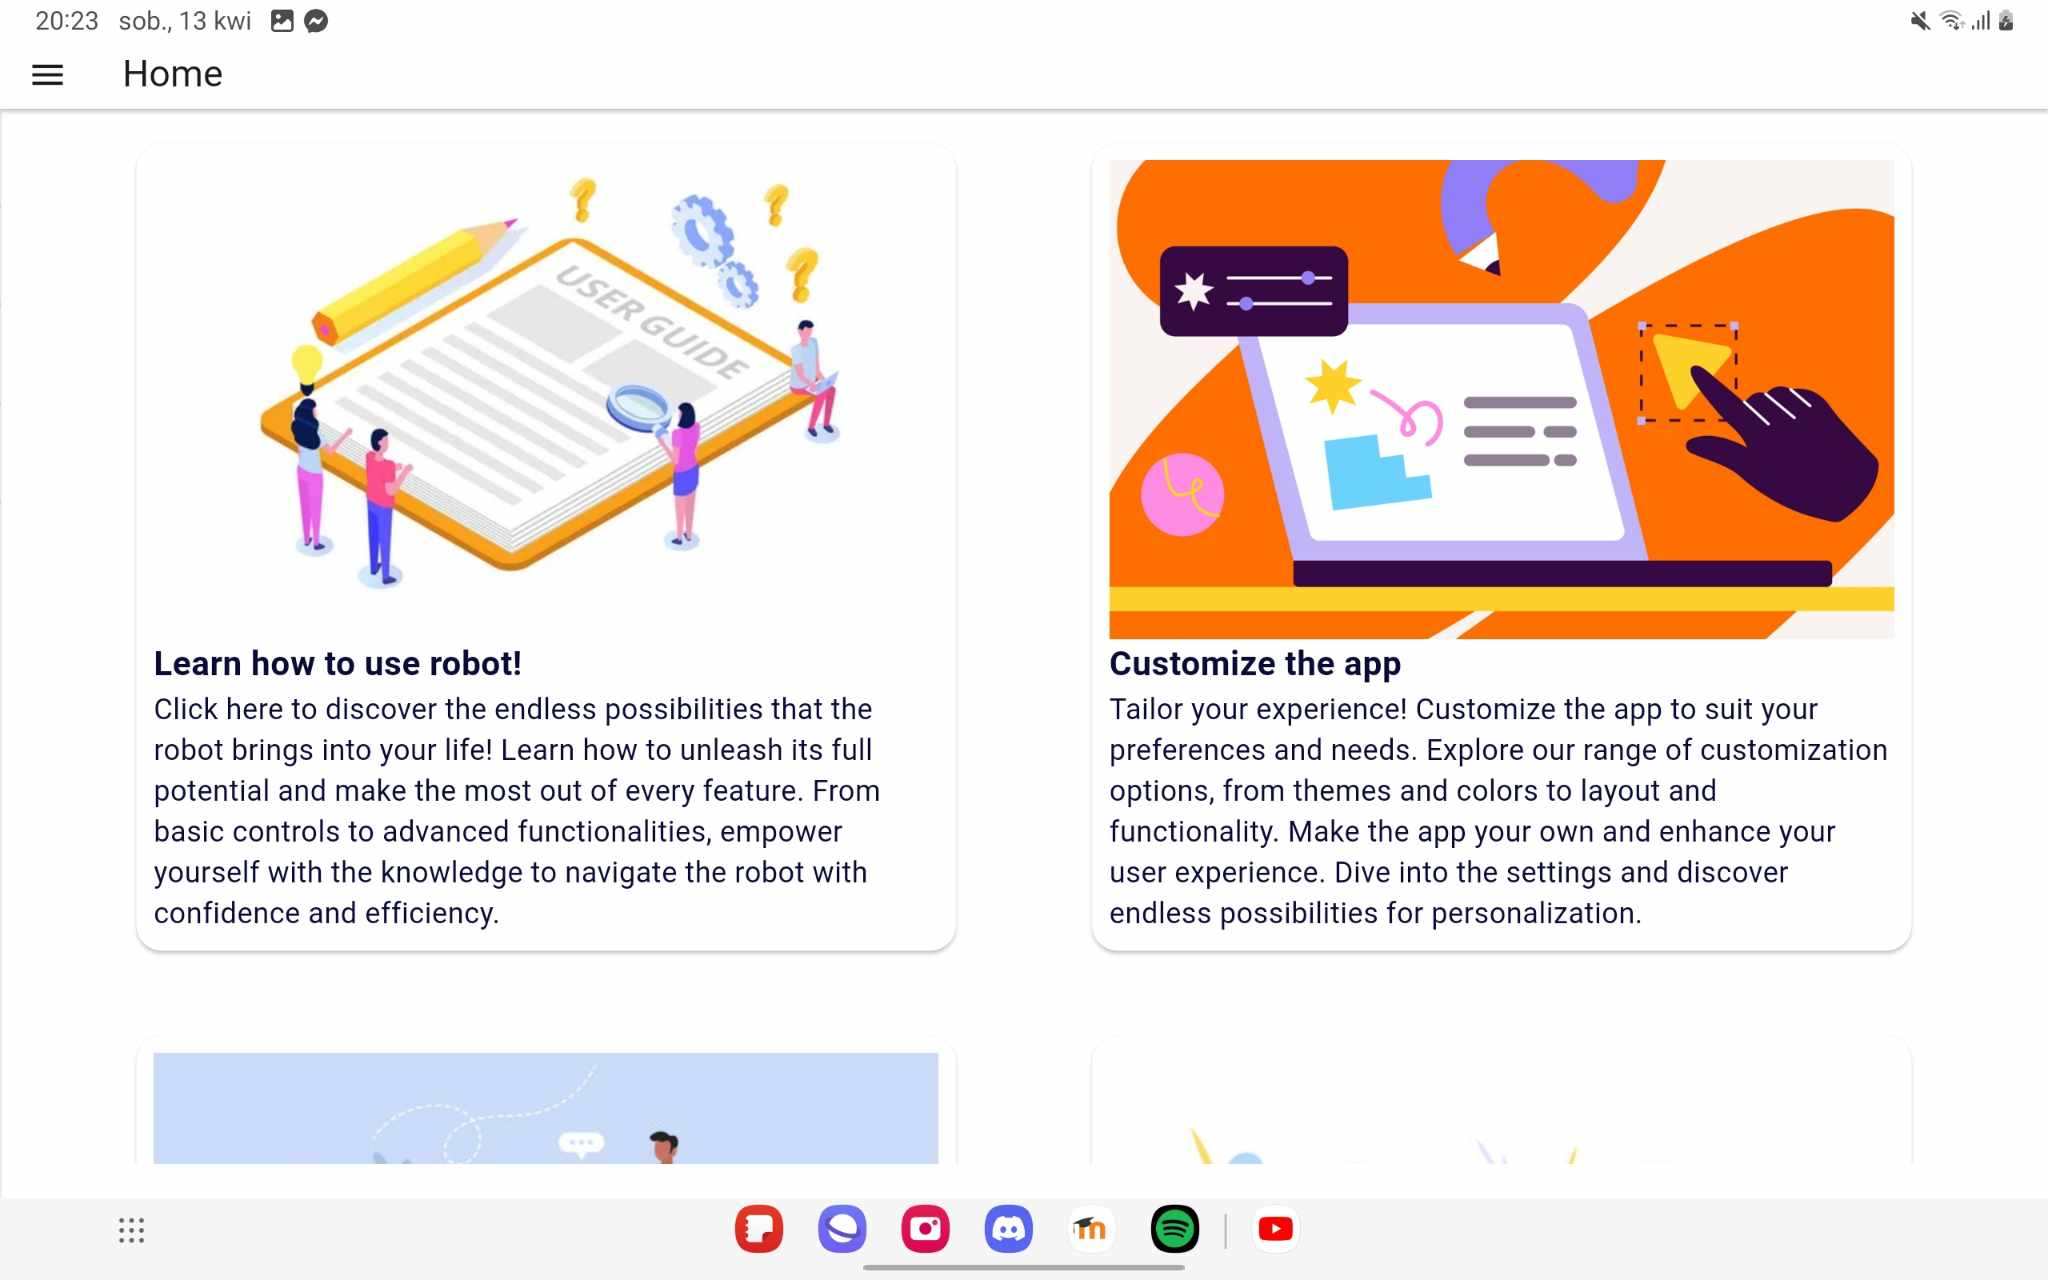
\includegraphics[width=1.0\textwidth]{src/app/home.jpg}
    \caption{Ekran początkowy aplikacji}
    \label{fig:home_screen}
\end{figure}

Trzecia i czwarta sekcja dotyczą genezy projektu oraz zespołu, który stworzył robota i aplikację. Ponadto, umożliwiają one użytkownikom przesyłanie opinii, co pozwala na wprowadzenie przyszłych aktualizacji mających na celu poprawę jakości korzystania z aplikacji.

\begin{figure}[H]
    \centering
    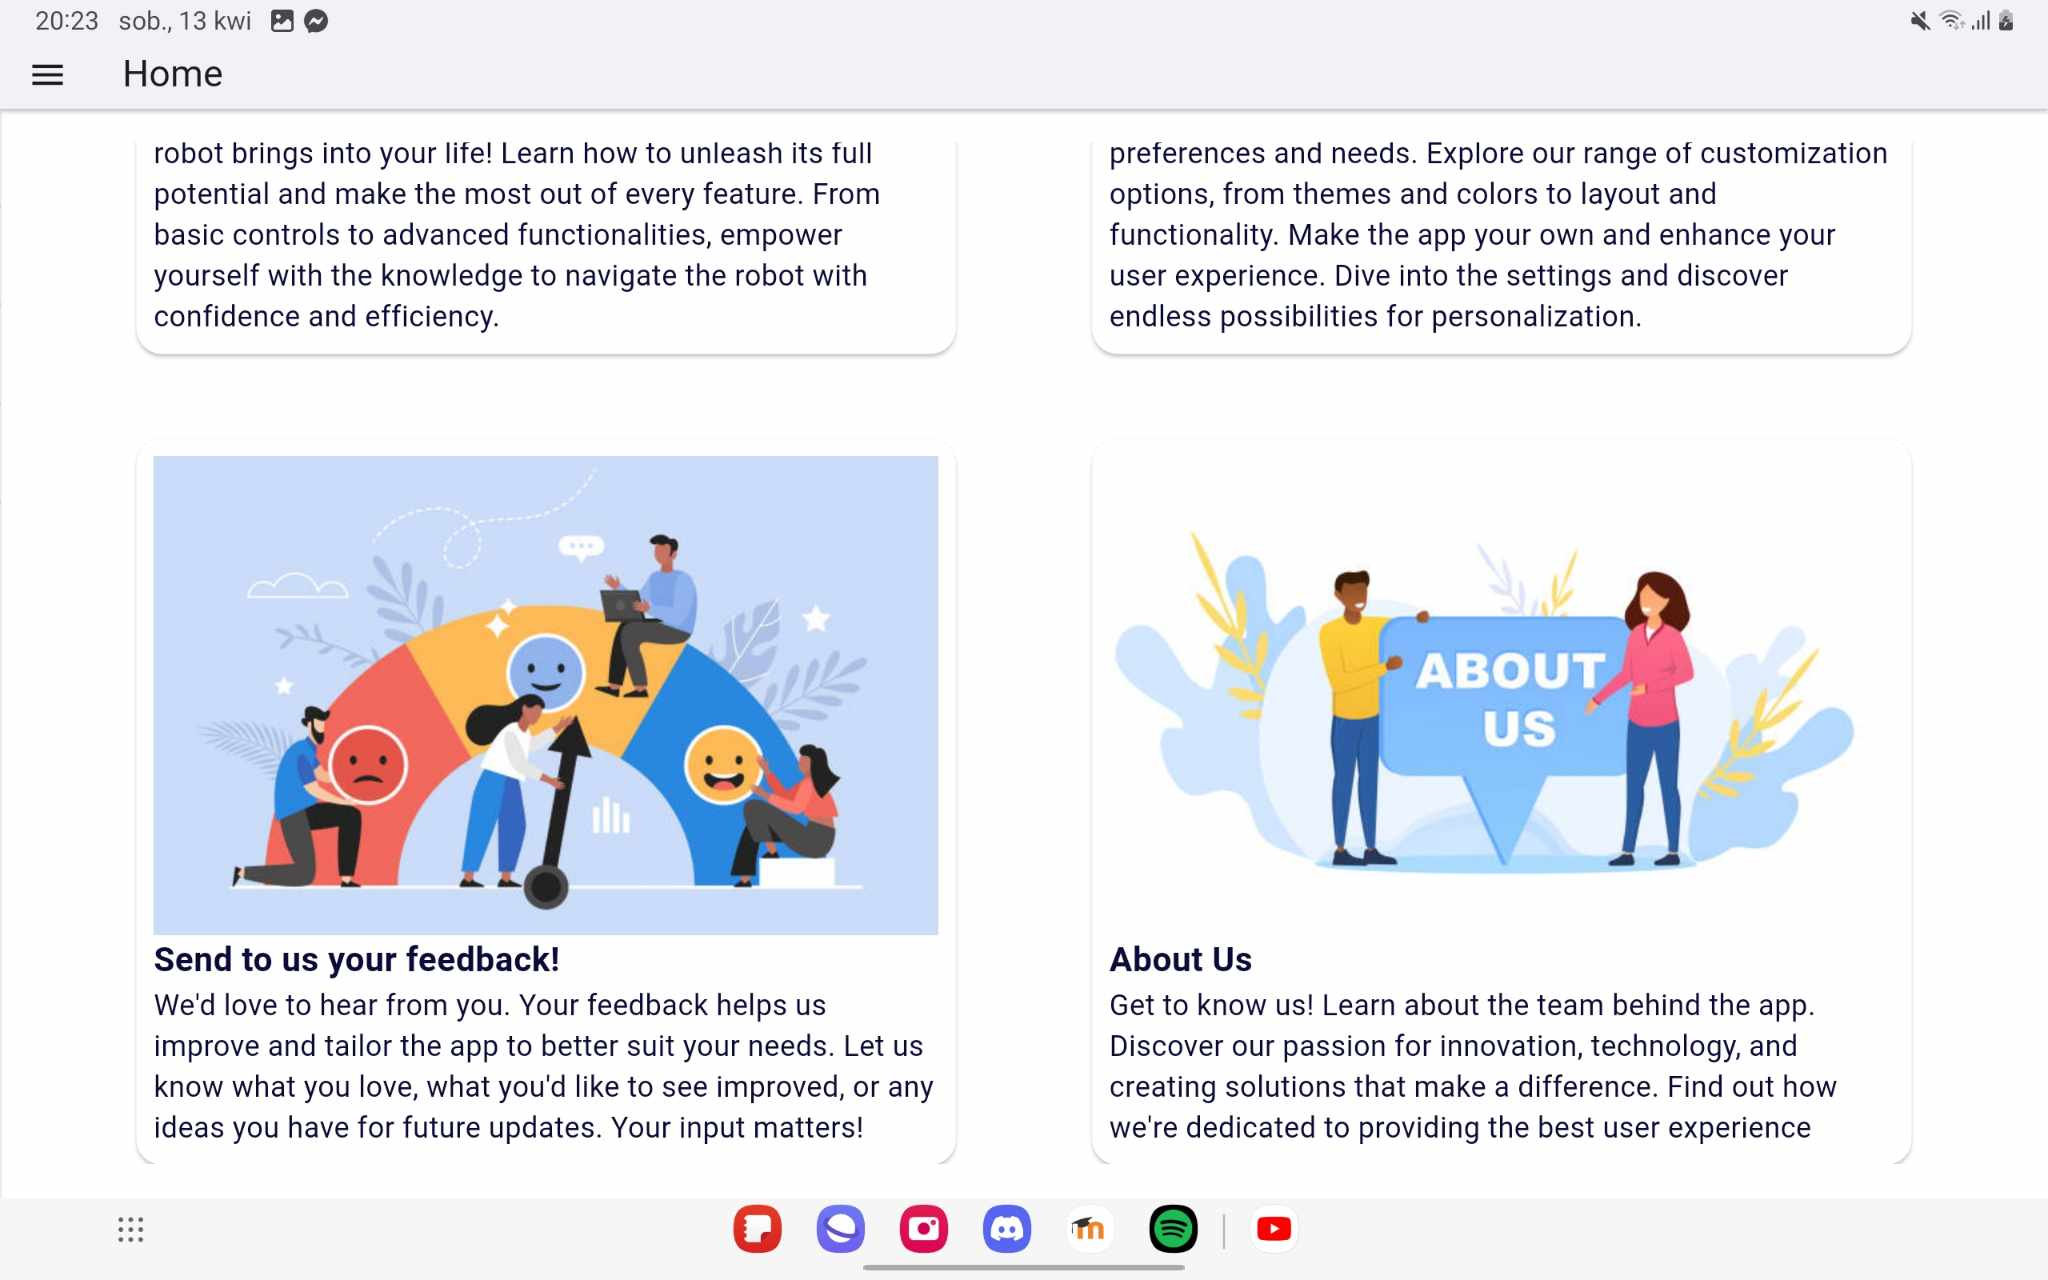
\includegraphics[width=1.0\textwidth]{src/app/home-2.jpg}
    \caption{Obraz prezentujący ekran początkowy aplikacji}
    \label{fig:home_screen-2}
\end{figure}

W lewym górnym rogu ekranu znajduje się standardowy dla aplikacji mobilnych przycisk rozwijający menu boczne. Menu zawiera wszystkie niezbędne zakładki, takie jak:
\begin{itemize}
\item \textit{Control Panel} (Panel Kontrolny) – umożliwia sterowanie robotem,
\item \textit{Connect to device} (Połącz z urządzeniem) – pozwala na wyszukiwanie i łączenie z urządzeniem,
\item \textit{Settings} (Ustawienia) – umożliwia dostosowanie parametrów robota,
\item \textit{Help} (Pomoc) – zawiera informacje o korzystaniu z aplikacji oraz dane kontaktowe działu wsparcia.
\end{itemize}

\begin{figure}[H]
    \centering
    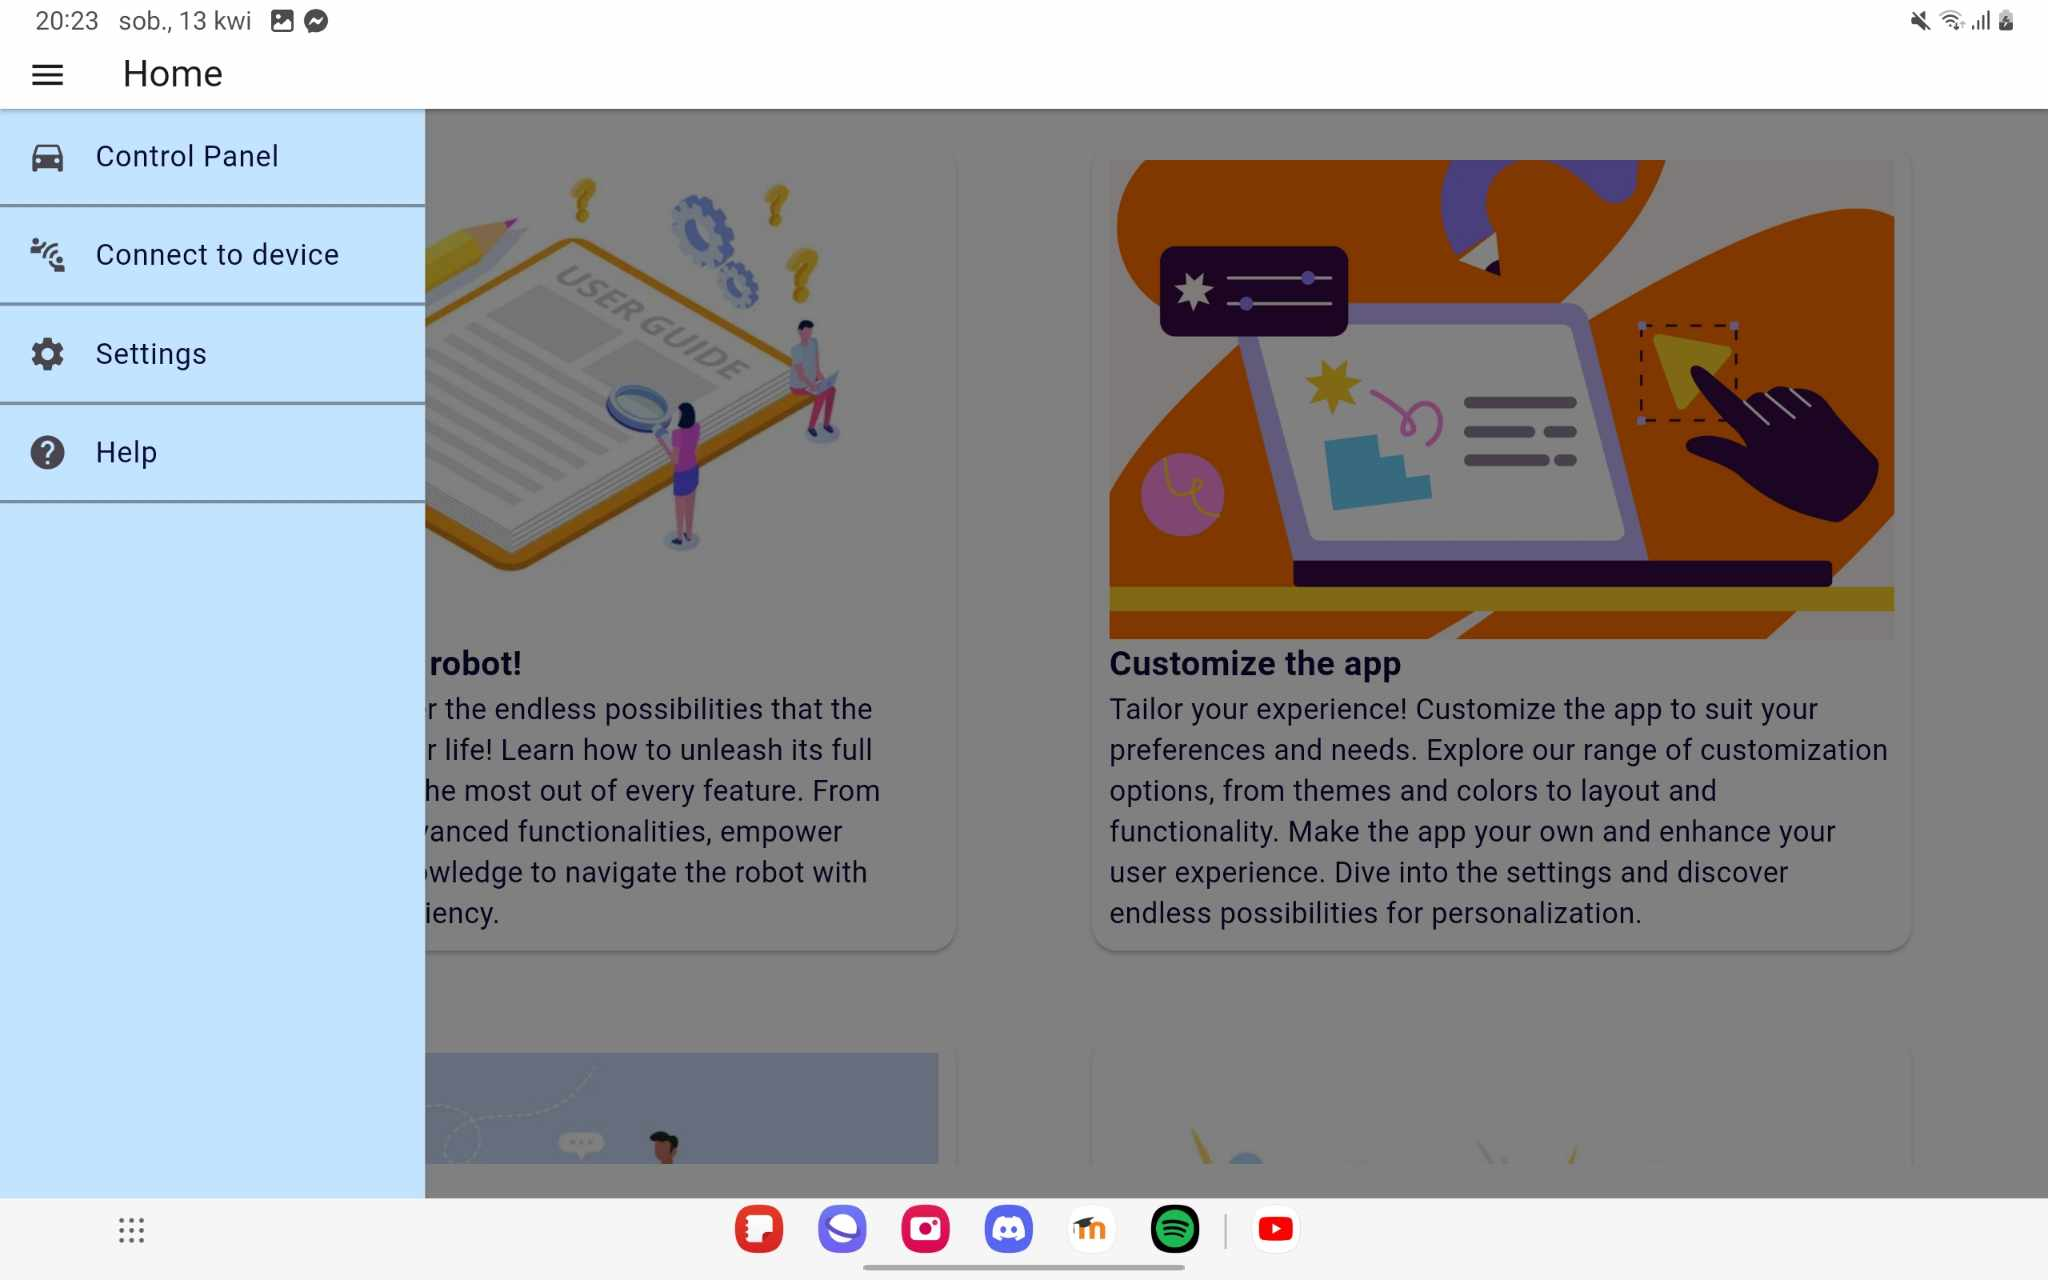
\includegraphics[width=1.0\textwidth]{src/app/tab-control.jpg}
    \caption{Menu boczne aplikacji}
    \label{fig:side-menu}
\end{figure}

Po kliknięciu w pierwszą zakładkę użytkownik zostaje przekierowany do strony odpowiedzialnej za sterowanie robotem. Ekran ten podzielony jest na dwie sekcje. Pierwsza z nich, zatytułowana \textit{Controls} (Kontrolki), umożliwia bezpośrednie sterowanie robotem poprzez odpowiednie przyciski. Po prawej stronie znajduje się sekcja, która w przyszłości ma wyświetlać animację przedstawiającą robota w ruchu.

\begin{figure}[H]
    \centering
    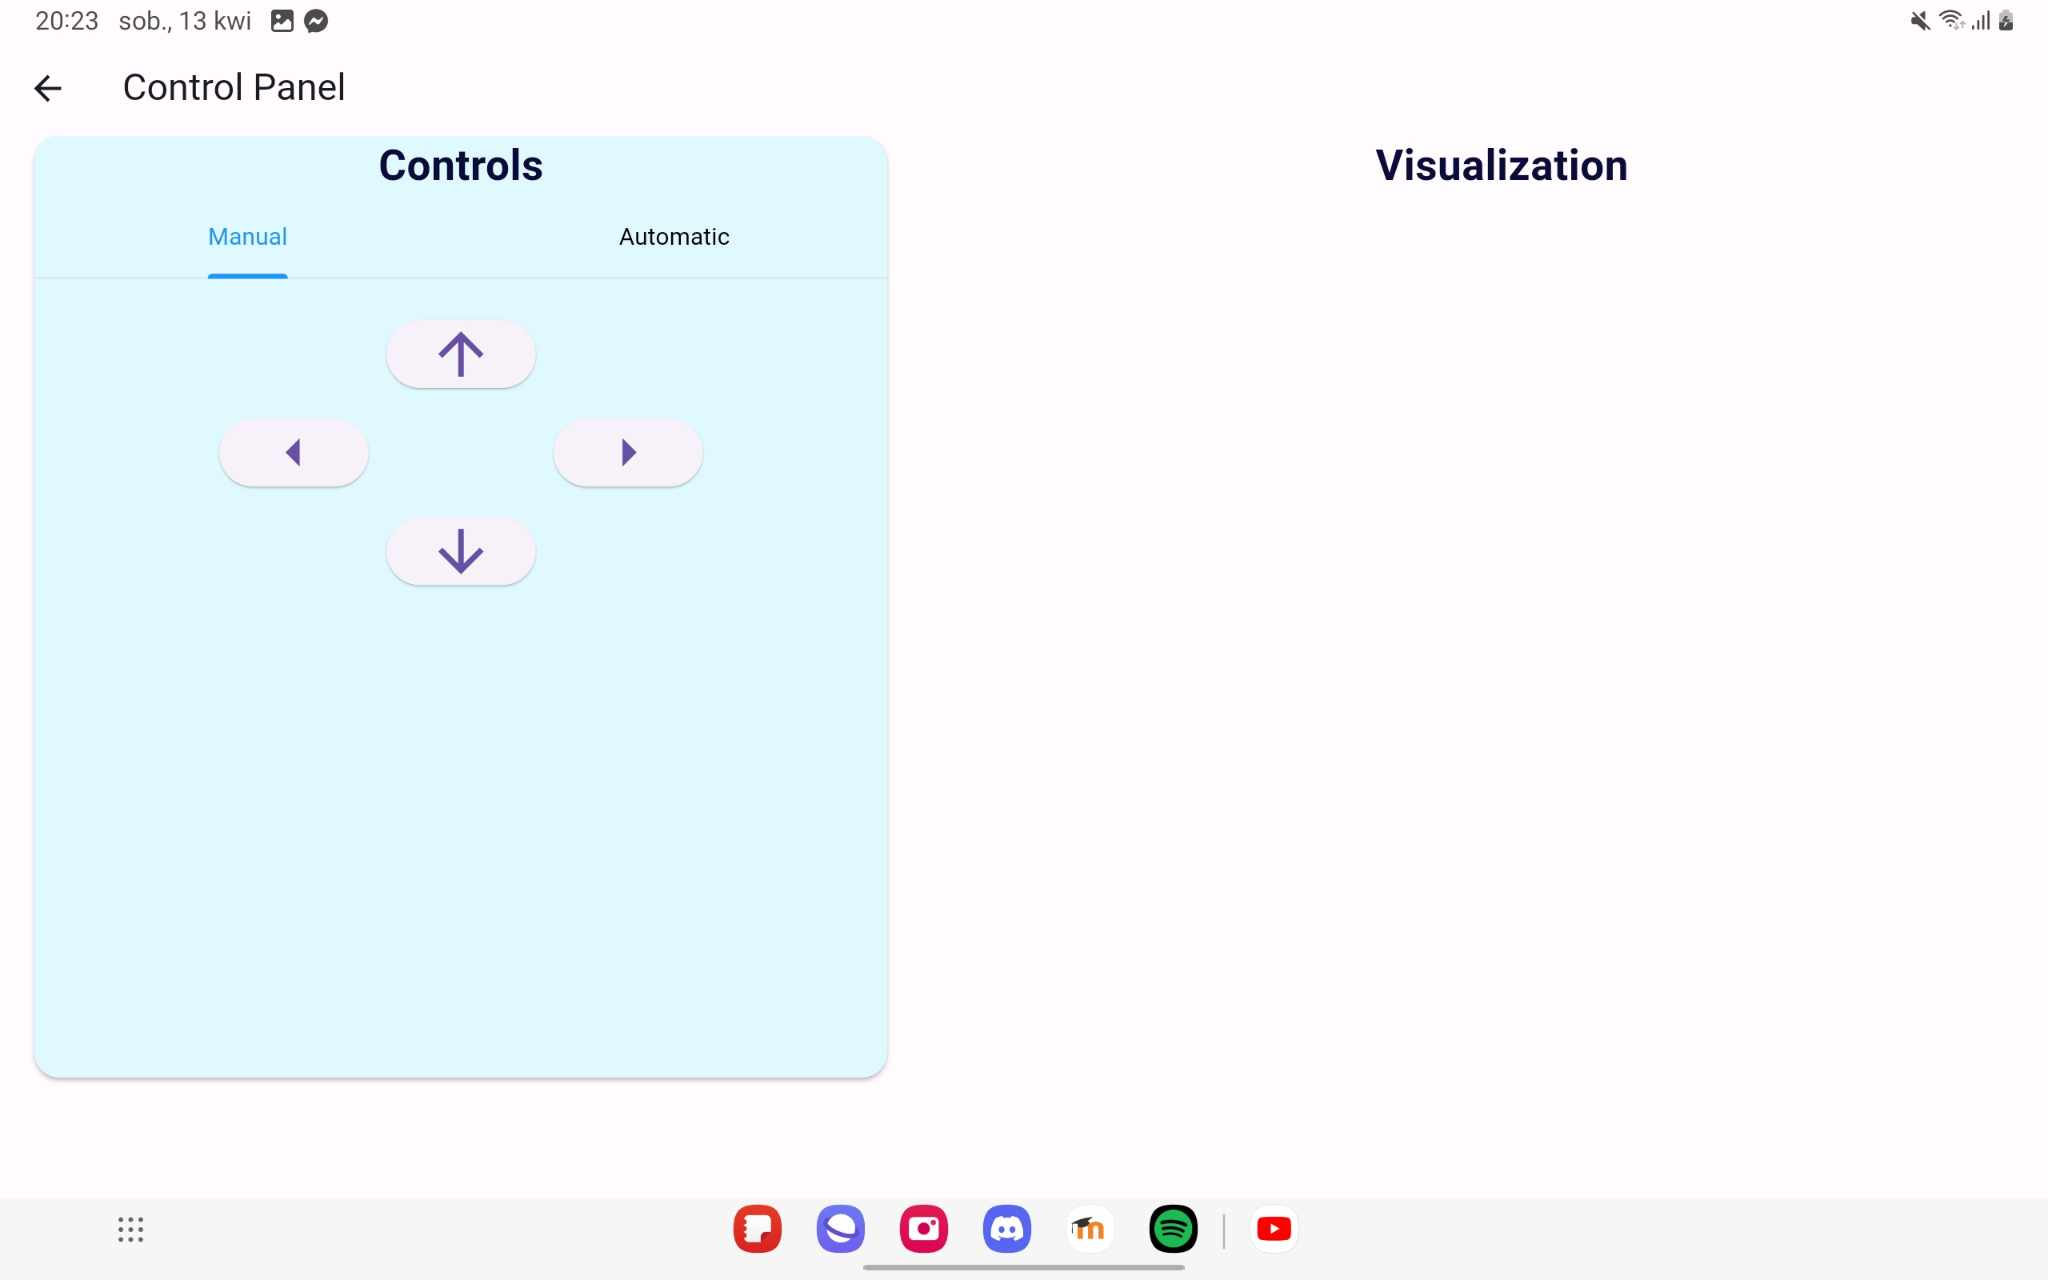
\includegraphics[width=1.0\textwidth]{src/app/control.jpg}
    \caption{Ekran kontroli robota}
    \label{fig:control}
\end{figure}

Kolejną zakładką jest ekran wyświetlający dostępne urządzenia Bluetooth. Użytkownik może połączyć aplikację z wybranym urządzeniem poprzez naciśnięcie przycisku \textit{Connect} (Połącz). Zaleca się łączenie wyłącznie z urządzeniami będącymi częścią systemu robota.

\begin{figure}[H]
    \centering
    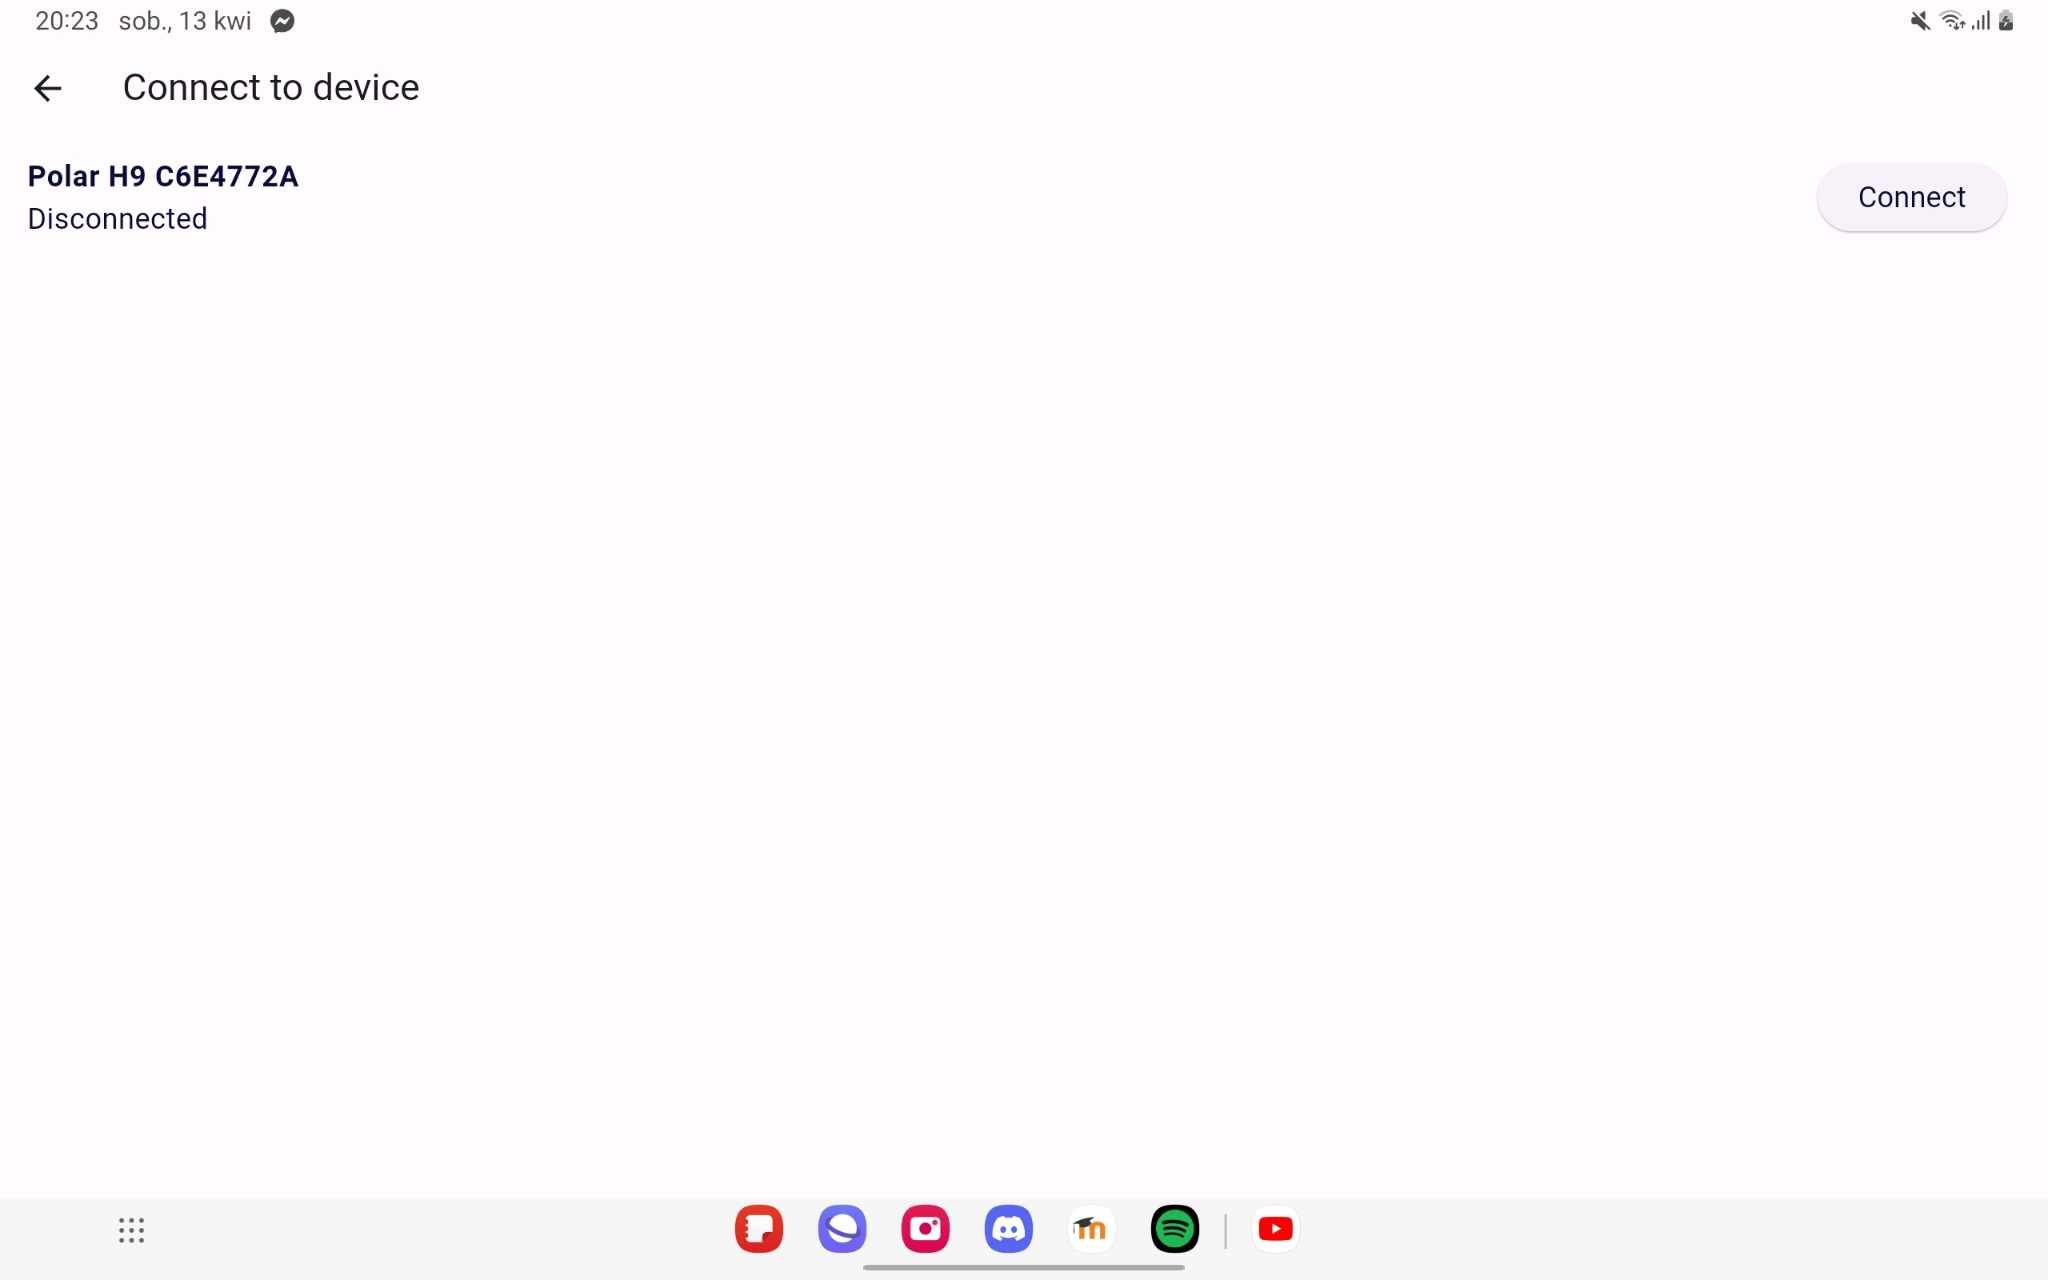
\includegraphics[width=1.0\textwidth]{src/app/list-devices.jpg}
    \caption{Ekran połączenia z urządzeniami}
    \label{fig:Connect}
\end{figure}

Zakładki takie jak \textit{Settings} (Ustawienia) i \textit{Help} (Pomoc) nie zostały zaimplementowane z powodu zmiany priorytetów podczas rozwoju projektu. Niemniej jednak, aplikacja ma duży potencjał rozwoju i może zostać rozbudowana w przyszłości.

\subsection{\Large Implementacja połączenia Bluetooth}
% --------------------------------------------------------
% Autor: Jakub Pajak
%
% TODO: Opisać zasadę działania połączenia Bluetooth poprzez paczkę flutter_blue
%
% Status: 100%
% --------------------------------------------------------

Kluczową informacją potrzebną do nawiązania połączenia z mikrokontrolerem Arduino UNO R4 jest fakt, iż mikrokontroler ten korzysta ze specyficznego rodzaju Bluetooth - Bluetooth Low Energy (BLE). W związku z tym konieczne było wykorzystanie odpowiedniej biblioteki, takiej jak \textit{flutter\_blue}. Bibliotekę tę można pobrać za pomocą narzędzia w terminalu, wpisując komendę:
\begin{verbatim}
flutter pub add flutter_blue
\end{verbatim}
Drugą istotną kwestią jest konieczność wykorzystania fizycznego urządzenia do uruchamiania aplikacji. Jest to zalecane ze względu na brak możliwości wyszukiwania urządzeń Bluetooth w niektórych emulatorach.


Pierwszym krokiem do nawiązania połączenia jest wyświetlenie listy wszystkich dostępnych urządzeń Bluetooth. W tym celu wykonywana jest funkcja \texttt{\_startScan()}, której zadaniem jest pobranie wszystkich dostępnych urządzeń i dodanie ich do listy w celu późniejszego wyświetlenia.

Funkcja \texttt{\_getPairedDevices()} zwraca wszystkie urządzenia, które zostały pomyślnie sparowane.

Po zakończeniu skanowania, proces jest zamykany przy pomocy funkcji \texttt{\_stopScan()}.

\begin{figure}[H]
    \centering
    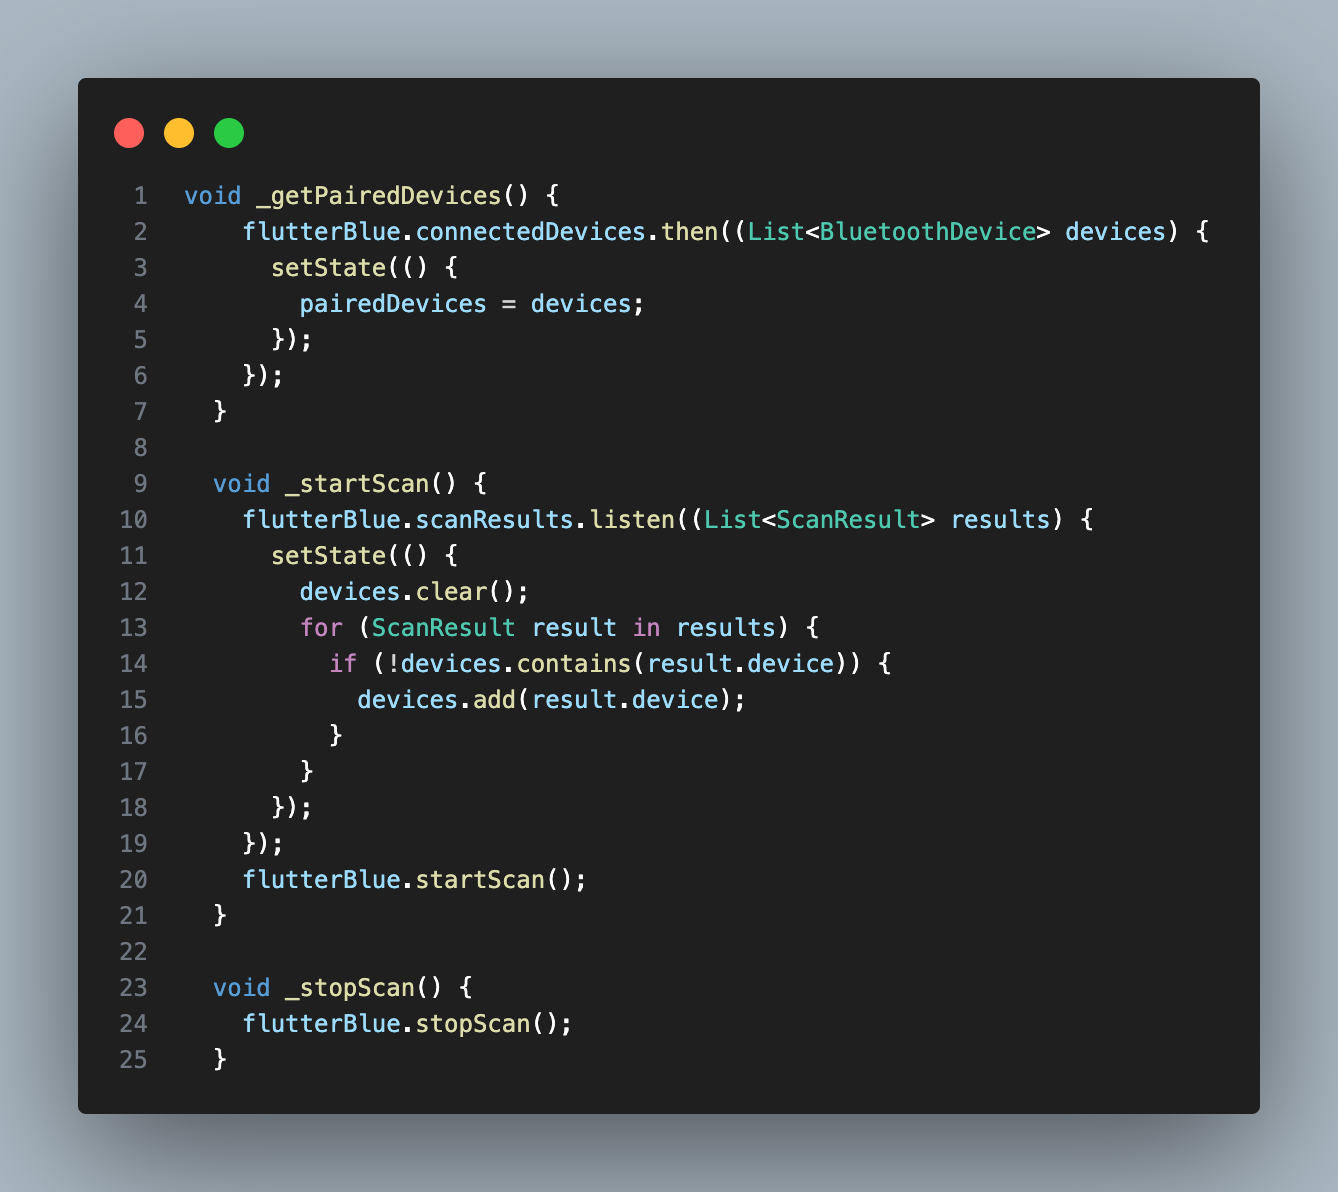
\includegraphics[width=0.7\textwidth]{src/app/_getPairedDeviced.png}
    \caption{Fragment kodu źródłowego zawierający implementację wyszukiwania dostępnych urządzeń}
    \label{fig:con-list}
\end{figure}

Kolejnym krokiem jest nawiązanie połączenia z wybranym urządzeniem. Proces ten jest realizowany przez funkcję \texttt{\_connectToDevice()}, która jako parametr przyjmuje referencję do wybranego urządzenia z listy. Funkcja ta wywołuje metodę kończącą skanowanie, a następnie na instancji klasy \texttt{BluetoothDevice} wywołuje metodę \texttt{connect()}, która realizuje połączenie. Klasa \texttt{BluetoothDevice} jest dostępna dzięki użyciu biblioteki \texttt{flutter\_blue}.

\begin{figure}[H]
    \centering
    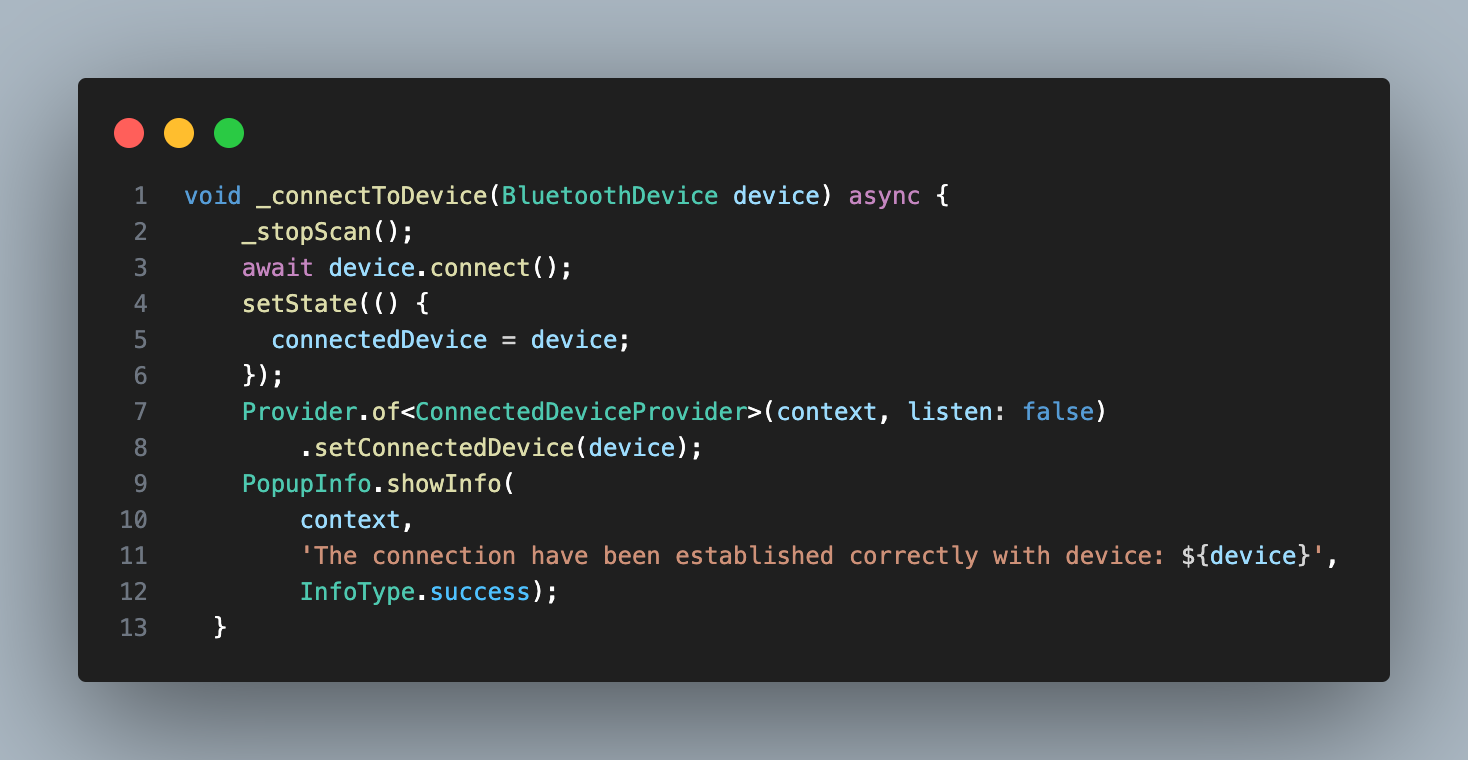
\includegraphics[width=0.7\textwidth]{src/app/connect.png}
    \caption{Fragment kodu źródłowego zawierający implementację nawiązywania połączenia BLE}
    \label{fig:con-soft}
\end{figure}


\subsection{\Large Implementacja przesyłania danych}
% --------------------------------------------------------
% Autor: Jakub Pajak
%
% TODO: Opisać sposób przekazywania infomracji o przyciśniętym przycisku w postaci całkowitoliczbowej
%
% Status: 100%
% --------------------------------------------------------

Proces przesyłania informacji do urządzenia Bluetooth opiera się na metodzie \texttt{sendValueToArduino()}. Ta metoda przyjmuje dwa parametry: referencję do połączonego urządzenia oraz wartość, która ma zostać przesłana.

Pierwszym krokiem w tej metodzie jest weryfikacja, czy urządzenie zostało poprawnie połączone oraz czy jest możliwe przesłanie danych. W przypadku niepowodzenia tej weryfikacji, w konsoli zostaje wyświetlona stosowna informacja diagnostyczna, co pozwala na szybkie zidentyfikowanie problemu.

Następnie metoda wyszukuje urządzenia o konkretnej charakterystyce, która jest niezbędna do prawidłowego funkcjonowania połączenia. Znalezienie urządzenia o odpowiedniej charakterystyce jest kluczowe, ponieważ zapewnia, że dane zostaną przesłane do właściwego odbiorcy.

Jeśli charakterystyka urządzenia zgadza się z oczekiwaną, wartość jest przesyłana. Taki proces zapewnia nie tylko prawidłowość przesyłania danych, ale również bezpieczeństwo połączenia.

Poniżej znajduje się fragment kodu źródłowego, który ilustruje implementację logiki przesyłania informacji do urządzenia.

\begin{figure}[H]
\centering
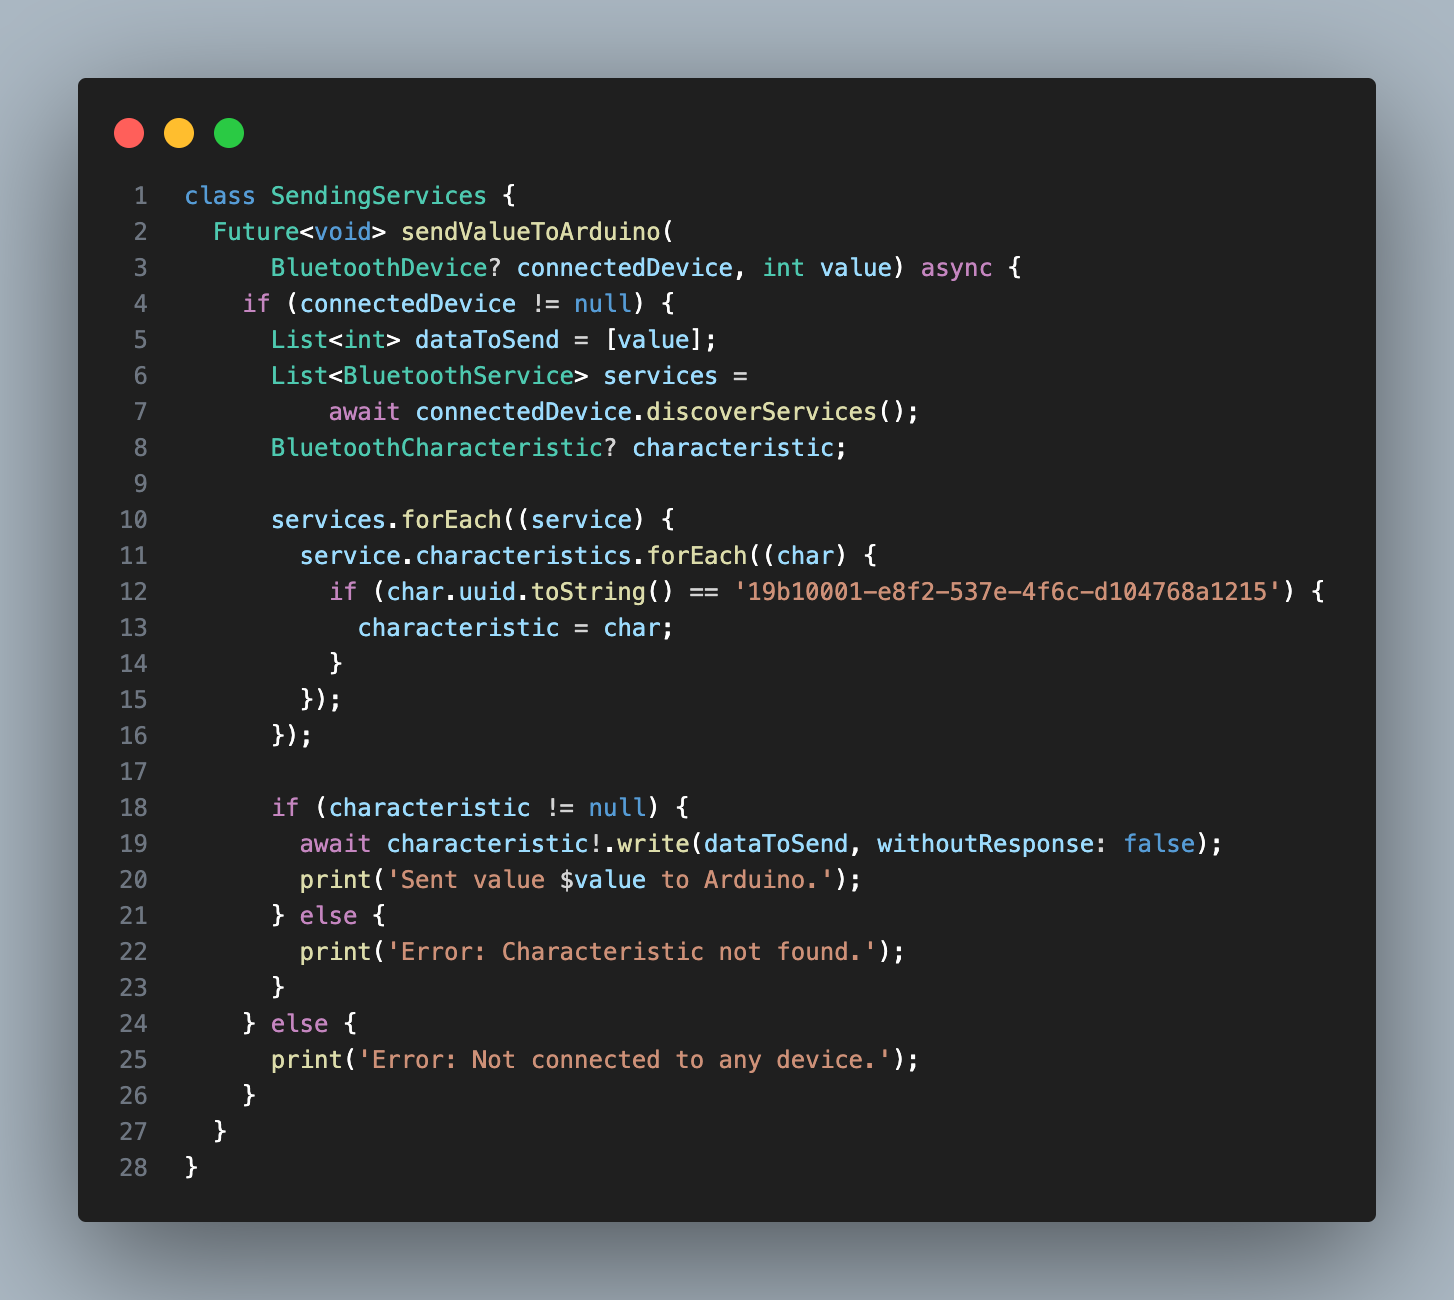
\includegraphics[width=0.7\textwidth]{src/app/send.png}
\caption{Fragment kodu źródłowego zawierający implementację logiki przesyłania informacji do urządzenia}
\label{fig:send-val}
\end{figure}


\subsection{\Large Implementacja prostego skryptu w odczytującego dane z kanału BLE }
Fragment prezentowanego kodu rozpoczyna się od zadeklarowania zmiennych globalnych opisujących charakterystyki połączenia Bluetooth. Pierwsza charakterystyka określa identyfikator typu GUID serwisu, następna określa na jaki identyfikator przesyłane są zdarzenia typu "request". Ostatnia wartość definiuje indentyfikator na jaki są przesyłane zdarzenia typu 'response". 
W przypadku aktualnej wersji aplikacji istotna jest tylko wartość identyfikująca serwis oraz zdarzenia typu request, ponieważ mikrokontroler nie zwraca żadnej informacji do aplikacji. W razie dalszego rozwoju projektu zostanie zaimplementowanie wyświetlanie diagnostyki robota, stanu naładowania baterii oraz stanu pracy silników. 

Funkcja \texttt{t5Callback()} ma za zadanie pobierać wartość która aktualnie została przesłana do kanału Bluetooth z poziomu aplikacji. Argumenty wejściowe funkcji to urządzenie z którym Arduino nawiązało połączenie, drugi argument to wcześniej wspomniany identyfikator zdarzenia "request".

Następnie wartość jest odczytywana z kanału za pomocą funkcji \texttt{readValue()}. Funkcja ta jest częścią biblioteki \texttt{ArduinoBLE.h}.

W funkcji \texttt{setup()} następuje inicjalizacja odpowiednich charakterystyk oraz za pomocą funkcji \newline \texttt{setEventHandler()} zostaje określona sytuacja w której nastąpi wywołanie funkcji \texttt{t5Callback} oraz odczytanie danych z kanału. 

\begin{figure}[H]
    \centering
    \includegraphics*[width=1.0\textwidth]{"src/code_snaps/bt_con_arduino.png"}
    \caption{Fragment kodu źródłowego przedstawiający implementację konfiguracji kanału Bluetooth na Arduino}
    \label{fig:bt_con_arduino}
\end{figure}


\newpage
\subsection{\Large Proces wykonywania projektu obudowy robota}
% --------------------------------------------------------
% Autor: Łukasz Grabarski
%
% TODO: Opisać proces oraz sposób wykonania projektu obudowy w 3D
%
% Status: 100%
% --------------------------------------------------------

Proces projektowania obudowy dla platformy jeżdżącej stanowił wieloetapowe zadanie, które wymagało dokładnego zaplanowania i licznych poprawek. Pierwsza faza obejmowała stworzenie prototypu, który miał na celu optymalne rozmieszczenie komponentów oraz weryfikację ich poprawnego działania. 
Ten etap pozwalał zidentyfikować ewentualne problemy konstrukcyjne i funkcjonalne na wczesnym etapie prac.

\begin{figure}[H]
    \centering
    \includegraphics*[width=0.4\textwidth]{"src/Robot_pics/Build_1.jpg"}
    \caption{Prototypowa konstrukcja mająca na celu sprawdzenie poprawności działania komponentów.}
    \label{fig:bt_con_arduino}
\end{figure}

Kolejnym krokiem było opracowanie specjalnej obudowy, zdolnej pomieścić wszystkie wymagane elementy, przy jednoczesnym zachowaniu odpowiedniej geometrii kół szwedzkich (zwanych również kołami Mecanum). 
Aby robot działał zgodnie z założeniami, koła musiały być rozmieszczone w orientacji X Y równych odstępach od siebie, a ich rolki powinny być skierowane do środka. Konieczne jest aby z rzutu górnego posiadał przedłużenie osi kół w kształcie znaku X. 


\begin{figure}[H]
    \centering
    \includegraphics*[width=0.5\textwidth]{"src/Robot_pics/Mecanum_lines.png"}
    \caption{Plan rozmieszczenia kół szwedzkich. Kluczowe jest zachowanie kół w równych odstępach od siebie oraz utworzenie znaku X.}
    \label{fig:bt_con_arduino}
\end{figure}


\begin{figure}[H]
    \centering
    \includegraphics*[width=1.0\textwidth]{"src/Robot_pics/blender.png"}
    \caption{Pierwsza wersja projektu zamodelowana w programie Blender 4.1.}
    \label{fig:bt_con_arduino}
\end{figure}

Jednakże podczas pierwszego etapu projektu nastąpiły problemy logiczne i konstrukcyjne. Pierwotnie używany darmowy program Blender 4.1 okazał się niewystarczający ze względu na niezgodność formatów eksportu z wymaganiami dostępnej drukarki 3D. 
W związku z tym, konieczne było przejście na bardziej zaawansowane narzędzie, jakim jest AutoDesk Fusion. To oprogramowanie pozwoliło na dokładniejsze zaprojektowanie modelu, uwzględniając specyfikację drukarki, która posiadała obszar roboczy o wymiarach 25 cm x 25 cm. 
Z tego powodu, model musiał zostać zaprojektowany od nowa, z uwzględnieniem ograniczeń.

\begin{figure}[H]
    \centering
    \includegraphics*[width=1.0\textwidth]{"src/Robot_pics/Fusion 1.png"}
    \caption{Wizualizacja gotowego modelu w programie AutoDesk Fusion.}
    \label{fig:bt_con_arduino}
\end{figure}

\newpage

Gotowy produkt składa się z dwóch pięter, z których każde pełni inną funkcje. 
Pierwsze piętro to "piętro maszynowe", gdzie umieszczone zostały moduły napędowe, takie jak silniki kątowe z przekładnia oraz ogniwa zasilające w ilości dwóch wraz ze sterownikiem BMS. 
Wszystkie istotne kable zostały przeprowadzone przez specjalnie przygotowany otwór do drugiego piętra.

\begin{figure}[htbp]
    \centering
    \begin{minipage}[b]{0.45\textwidth}
        \centering
        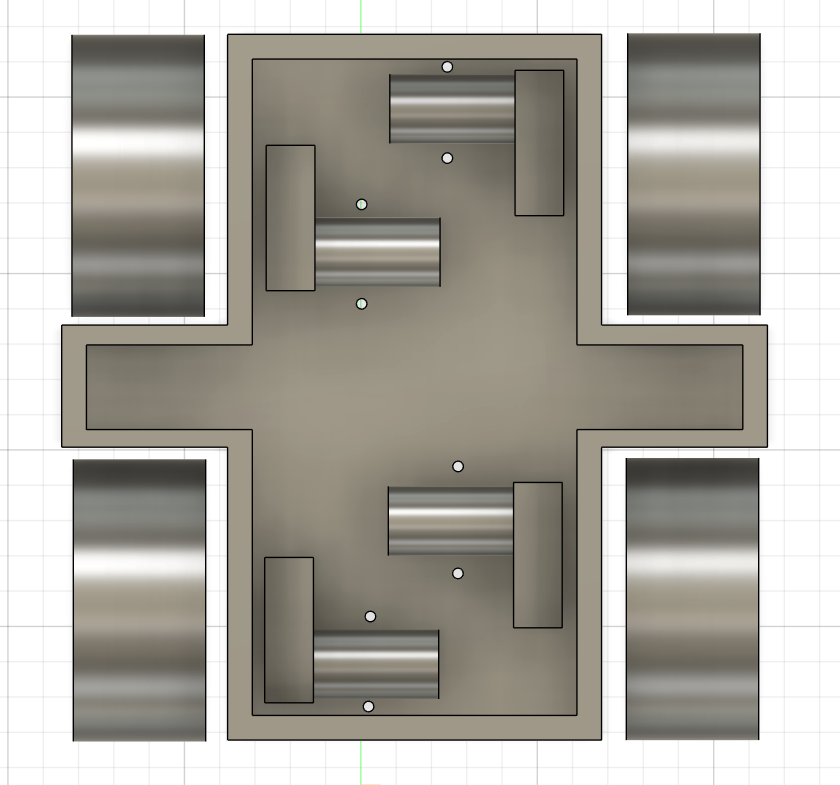
\includegraphics[width=\textwidth]{src/Robot_pics/Dol.png}
        \caption{Widok rzutu górnego na pierwsze piętro modelu. Znajdują się w nim silniki kątowe z przekładnią oraz miejsce na ogniwa zasilające wraz z BMS.}
        \label{fig:zdjecie1-robo}
    \end{minipage}
    \hfill
    \begin{minipage}[b]{0.45\textwidth}
        \centering
        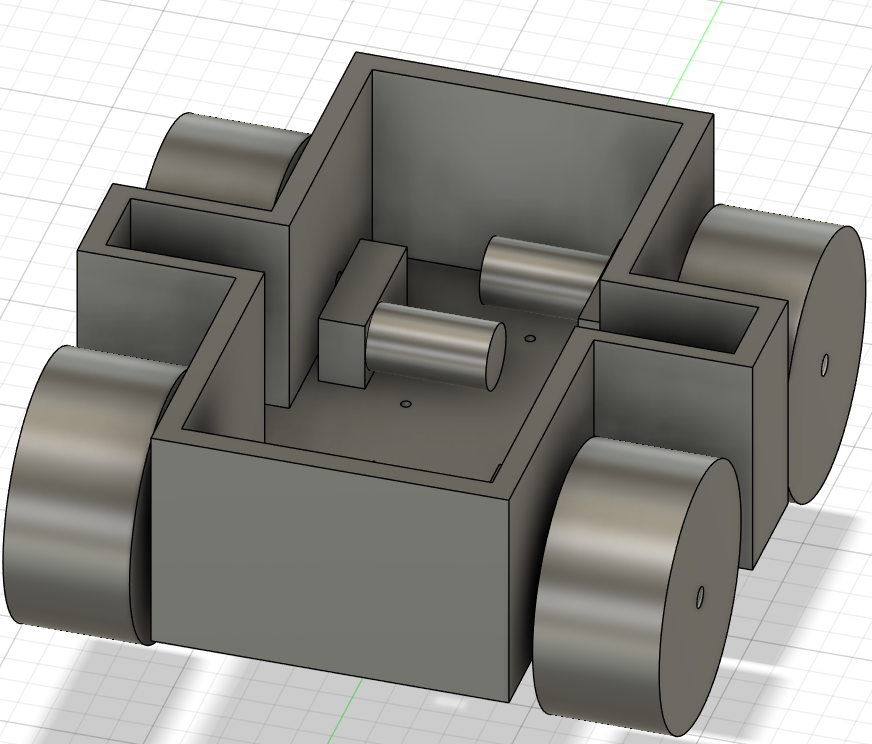
\includegraphics[width=\textwidth]{src/Robot_pics/Dol 1.png}
        \caption{Widok rzutu bocznego na pierwsze piętro modelu.}
        \label{fig:zdjecie2}
    \end{minipage}
\end{figure}

Drugie piętro to "mózg operacyjny" całego projektu. Zawiera ono kluczowe połączenia elektroniczne, w tym dwa mikrokontrolery Arduino UNO 4 i 3 w konfiguracji Master-Slave, oraz osiem czujników laserowych umieszczonych w przygotowanych otworach na ścianach bocznych. 
Takie rozmieszczenie i organizacja komponentów pozwalają na efektywne zarządzanie funkcjami robota.

\begin{figure}[htbp]
    \centering
    \begin{minipage}[b]{0.45\textwidth}
        \centering
        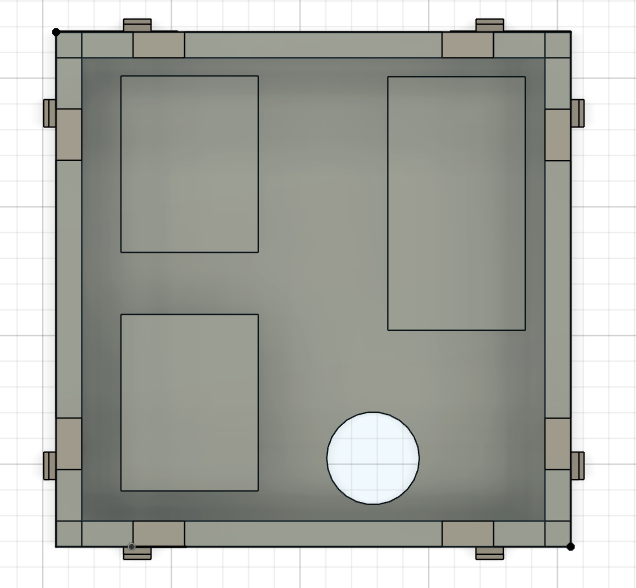
\includegraphics[width=\textwidth]{"src/Robot_pics/Gora.png"}
        \caption{Widok rzutu górnego na drugie piętro modelu. Znajdują się w nim dwa mikronotrolery Arduino UNO oraz płytka stykowa.}
        \label{fig:zdjecie1}
    \end{minipage}
    \hfill
    \begin{minipage}[b]{0.45\textwidth}
        \centering
        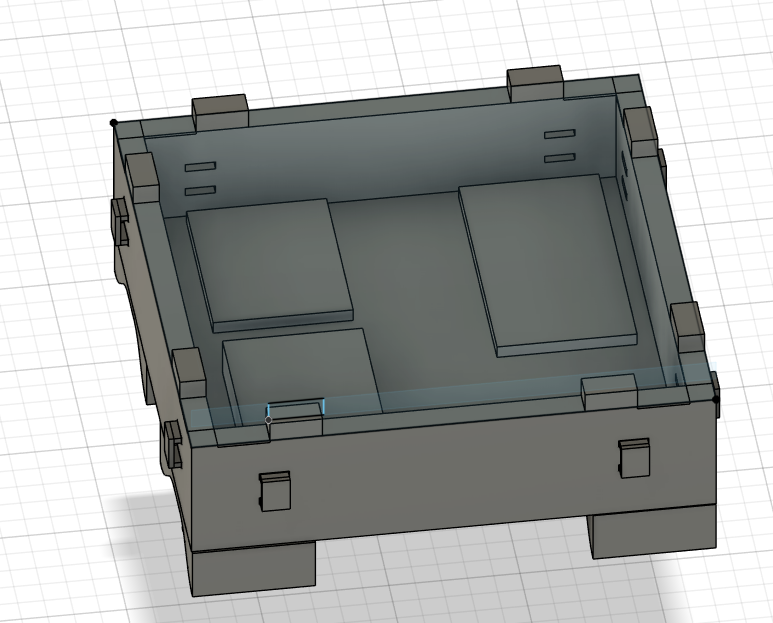
\includegraphics[width=\textwidth]{"src/Robot_pics/Gora 1.png"}
        \caption{Widok rzutu bocznego na drugie piętro modelu.}
        \label{fig:zdjecie2}
    \end{minipage}
\end{figure}

\begin{figure}[H]
    \centering
    \includegraphics*[width=1.0\textwidth]{"src/Robot_pics/Fusion 3.png"}
    \caption{Widok rzutu bocznego na specjalnie przygotowane miejsca do wsunięcia czujników laserowych.}
    \label{fig:bt_con_arduino}
\end{figure}

\begin{figure}[H]
    \centering
    \includegraphics*[width=1.0\textwidth]{"src/Robot_pics/Fusion 2.png"}
    \caption{Gotowy model przesłany do wydruku. Został pozbawiony elementów stylistycznych takich jak koła, silniki kątowe, mikrokontrolerów Arduino UNO oraz czujników laserowych.} 
    \label{fig:bt_con_arduino}
\end{figure}

\newpage

Gotowy model zawiera się w wymiarach 20 cm x 20 cm x 15 cm oraz wykonuje wszystkie zadane ruchy zdolne do wykonania tylko przy pomocy
kół szwedzkich. Pojazd wykonuje jazdę w kierunku w przód i w tył oraz w lewo i w prawo jak i obrót w miejscu.

\begin{figure}[H]
    \centering
    \includegraphics*[width=0.5\textwidth]{"src/Robot_pics/Finished.png"}
    \caption{Gotowy model po złożeniu wszystkich elementów w całość.}
    \label{fig:bt_con_arduino}
\end{figure}



\subsection{\Large Implementacja prostego kodu weryfikującego prawidłowe podłączenie silników}

% --------------------------------------------------------
% Autor: Krzysztof Grądek
%
% TODO: Opisać kod oraz sposób podłączenia silników do sterownika + krótki opis sterownika
%
% Status: 100%
% --------------------------------------------------------

Do połączenia silników z Arduino wykorzystano nakładkę Iduino ST1138. Umożliwia ona sterowanie czterema silnikami prądu stałego, o poborze prądu do 600 mA i napięciu zasilania do 36 V. Nakładka jest zasilana dwoma ogniwami 18650.

Weryfikacja połączenia silników została wykonana przy użyciu skryptu zamieszczonego poniżej. Na początku skryptu dodane są biblioteki Wire i AFMotor. Biblioteka Wire jest wykorzystywana do połączenia obu modułów Arduino w konfiguracji master-slave, natomiast biblioteka AFMotor służy do sterowania silnikami z nakładki Iduino.

W następnych liniach zdefiniowane są: adres urządzenia slave oraz globalna wartość bezpiecznego dystansu, który jest potrzebny, aby w przypadku wystającego gzymsu, który mógłby ominąć czujniki, pojazd nie zahaczył o niego.

Dalsza część kodu zawiera wykorzystanie biblioteki AFMotor i przypisanie konkretnych silników do zmiennych.

W ostatniej części, czyli setup, znajduje się połączenie przez bibliotekę Wire, rozpoczęcie komunikacji z prędkością 9600 bitów na sekundę (Serial.begin(9600)) oraz ustawienie prędkości wszystkich silników.

Do weryfikacji działania silników można zakomentować pozostałe ustawienia setSpeed, tak aby pozostało tylko jedno i sprawdzić, który silnik jest uruchomiony.
\begin{figure}[H]
    \centering
    \includegraphics*[width=1.0\textwidth]{"src/code_snaps/eng_ste_arduino.png"}
    \caption{Framgent kodu źródłowego przedstawiający weryfikacje prawidłowego połączenia silników}
    \label{fig:eng_ste_arduino}
\end{figure}

\subsection{\Large Podłączenie oraz weryfikacja poprawności działania czujników laserowych}

% --------------------------------------------------------
% Autor: Jakub Pająk
%
% TODO: Opisać sposób podłączenia czujników oraz kod weryfikujący podłączenie
%
% Status: 100% done
% --------------------------------------------------------
We wczesnej fazie planowania zakładano wykorzystanie ultradźwiękowych czujników odległości. Pomysł ten okazał się nietrafiony ze względu na sposób przekazywania danych przez te czujniki. Każdy czujnik posiada dwa wyprowadzenia, co przy użyciu ośmiu czujników wymagałoby wykorzystania co najmniej 16 pinów Arduino.

Następnie analiza skupiła się na wykorzystaniu magistrali I2C, która umożliwia podłączenie dużej liczby czujników za pomocą niewielkiej liczby pinów. Kluczowym warunkiem jest poprawna komunikacja między czujnikiem a mikrokontrolerem.

Laserowe czujniki odległości VL530L0X okazały się trafnym wyborem ze względu na ich korzystny stosunek jakości do ceny. Pomiary odległości są wystarczająco dokładne, a biorąc pod uwagę charakter obiektu wykrywanego, wysoka precyzja nie jest wymagana.

Czujniki zostały podłączone zgodnie z przeznaczeniem poprzez magistralę I2C. Kluczową rolę w podłączaniu wielu identycznych czujników odegrało użycie dodatkowego pinu XSHUT oraz odpowiedniej sekwencji kodu, aby pomyślnie zmienić adres czujnika na magistrali I2C. 

Pierwszym krokiem jest ustawienie odpowiedniego pinu GPIO (ang. General Purpose Input/Output) Arduino, podłączonego do pinu XSHUT czujnika, w trybie OUTPUT. Następnie należy skorzystać z funkcji \texttt{setAddress()}, aby ustawić odpowiedni adres dla wybranego czujnika. Kolejnym krokiem jest przełączenie stanu pinu Arduino na INPUT oraz odczekanie 10 milisekund.

Wykonanie powyższej sekwencji gwarantuje poprawną zmianę adresu czujnika na magistrali I2C. Użycie samej funkcji \texttt{setAddress()} bez zastosowania pinu XSHUT nie zmieni adresu czujnika.

\begin{figure}[H]
    \centering
    \includegraphics*[width=0.5\textwidth]{"src/code_snaps/sensor_init.png"}
    \caption{Fragment kodu źródłowego przedstawiający sekwencję konieczną do zmiany adresu czujnika}
    \label{fig:sensor_init}
\end{figure}


\subsection{\Large Montaż silników wewnątrz dolnej komory obudowy}

% --------------------------------------------------------
% Autor: Piotr Legień && Krzysztof Grądek
%
% TODO: Opisać sposób montażu silników oraz usztywnienia wału silnika + montaż kół
%
% Status: 90%
% --------------------------------------------------------
Silniki zostały przymocowane do dolnej części pojazdu za pomocą taśmy aluminiowej. Po wykonaniu tego kroku, przystąpiono do montażu kół na silnikach. Koła zostały zamontowane na wygwintowanej szprysze, która została przymocowana bezpośrednio do silników.

W celu wyeliminowania luzów na silnikach, podjęto dodatkowe działania. Wycięto dwie listwy aluminiowe, które zamontowano w taki sposób, aby przez nie przechodziły szprychy. Dzięki zastosowaniu tych listew, luz na kołach został znacznie zminimalizowany, co zapewniło stabilność całej konstrukcji.

Wykonanie tych czynności pozwoliło na usztywnienie wału silnika i zapewniło solidne połączenie kół z silnikami.
\begin{figure}[H]
    \centering
    \includegraphics*[width=0.5\textwidth]{"src/Robot_pics/listwa-kola.jpg"}
    \caption{Listwa boczna usztywniająca mocowanie silnika i eliminująca luzy na kole.}
    \label{fig:listwa-kola}
\end{figure}

\subsection{\Large Montaż ogniw wraz z układem BMS oraz podłączenie czujników}

% --------------------------------------------------------
% Autor: Bartosz Wuwer && Piotr Legień
%
% TODO: Opisać sposób połączenia ogniw oraz układ BMS (po co jest etc.)
%
% Status: 
% --------------------------------------------------------

\newpage
\subsection{\Large Integracja czujników z silnikami oraz implementacja logiki sterowania}
% --------------------------------------------------------
% Autor: Jakub Pająk && Łukasz Grabarski
%
% TODO: Opisać kod implementujący integrację czujników z silnikami
%
% Status: Łukasz 50% (jeszcze coś dopiszę)
% --------------------------------------------------------

W celu osiągnięcia optymalnej integracji modułu czujników oraz modułu sterowania silnikami zastosowano strukturę opartą na magistrali I2C. W omawianym układzie wykorzystano architekturę typu Master-Slave. Moduł odczytu danych z czujników oraz moduł odpowiedzialny za sterowanie silnikami są realizowane przez dwa oddzielne mikrokontrolery Arduino UNO. Mikrokontroler odpowiedzialny za odczyt wartości z czujników pełni rolę Master, przetwarzając informacje uzyskane z czujników i na ich podstawie przesyłając sygnały sterujące do mikrokontrolera pełniącego rolę Slave.

Zastosowanie tej specyficznej architektury było niezbędne z uwagi na ograniczenia w dostępności pinów GPIO. Wykorzystanie czterokanałowego sterownika silników w formie nakładki na mikrokontroler Arduino spowodowało zmniejszenie liczby dostępnych pinów do pinów analogowych o adresach od A0 do A5. Jak wspomniano w sekcji 2.8, wykorzystanie kilku czujników wymaga dostosowania ich adresów. W związku z tym konieczne było uzyskanie dostępu do co najmniej siedmiu pinów ogólnego przeznaczenia I/O, co zapewnia drugie Arduino pełniące rolę Master.

\subsubsection{\large Master}

Kod źródłowy rozpoczyna się od deklaracji oraz inicjalizacji zmiennych oraz stałych globalnych. Są to między innymi adresy czujników, typ wyliczeniowy zawierający informacje o aktualnej trajektorii robota oraz adresy pinów do których zostaną podłączone piny XSHUT. 

Następnie w funkcji \texttt{setup()} wykonywana jest inicjalizacja czujników. Proces inicjalizacji rozpoczyna się od ustawienia odpowiedniego adresu dla każdego czujnika. Proces ten został opisany wcześniej. Kolejnym etapem jest właściwa inicjalizacja czujnika. Wykonywana jest ona za pomocą funkcji \texttt{init()} wywoływanej na każdej instancji obiektu czujnika. W przypadku błędnej inicjalizacji wyświetlany jest stosowny komunikat. Następnie dla każdego czujnika ustawiany jest czas maksymalnego oczekiwania na wartość (ang. timeout) za pomocą funkcji \texttt{setTimeout()}. Jest on ustawiony na wartość 500ms, zatem po tym czasie zostanie zwrócona wartość maksymalna dla typu UINT16. Ostanim zadaniem jest przełączenia czujnika w tryb odczytu ciągłęgo za pomocą funkcji \texttt{setContinuous()}.


Następna funkcja typowa dla środowiska Arduino IDE to \texttt{setup()}. Funkcja ta zawiera wywołania czterech dodatkowych funkcji:
\begin{itemize}
    \item \texttt{searchForDevices()} - odpowiada za wyszukiwanie dostępnych urządzeń na magistrali I2C,
    \item \texttt{readFromSensor()} - odpowiada za odczytanie wartości z czujników,
    \item \texttt{processSensorInfo()} - odpowiada za interpretację otrzymanych wyników,
    \item \texttt{sendSteering()} - odpowiada za przesłanie instrukcji sterowania do urządzenia Slave.
\end{itemize}

\subsubsection*{Funkcja \texttt{searchForDevices()}}

Funkcja ta jest funkcją pomocniczą, niekonieczną do poprawnego działania programu. Jest ona jedna przydatna w celu weryfikacji poprawności połączenia urządzeń do magistrali I2C. W przypadku braku dostępnych urządzeń lub braku zgodności ich liczby należy zwrócić uwagę, czy wszystkie urządzenia są poprawnie podłączone do zasilania oraz do magistrali. Jeśli pierwsze w kolejności urządzenie podłączone do magistrali jest wadliwe lub zostało niepoprawnie podłączone, żadne kolejne urządzenie nie zostanie wykryte. 


Realizacja wyszukiwania dostępnych urządzeń (adresów) jest relatywnie prosta. W pętli \texttt{for} poprzez wywołanie funckji \texttt{Wire.beginTransmission(int addr)} rozpoczynana jest próbna transmisja do potencjalnego urządzenia. Jeśli urzadzenie odpowie bez błędu, jego adres jest wyświelany w konsoli w postaci liczby w formacie szesnastkowym.
\begin{figure}[H]
    \centering
    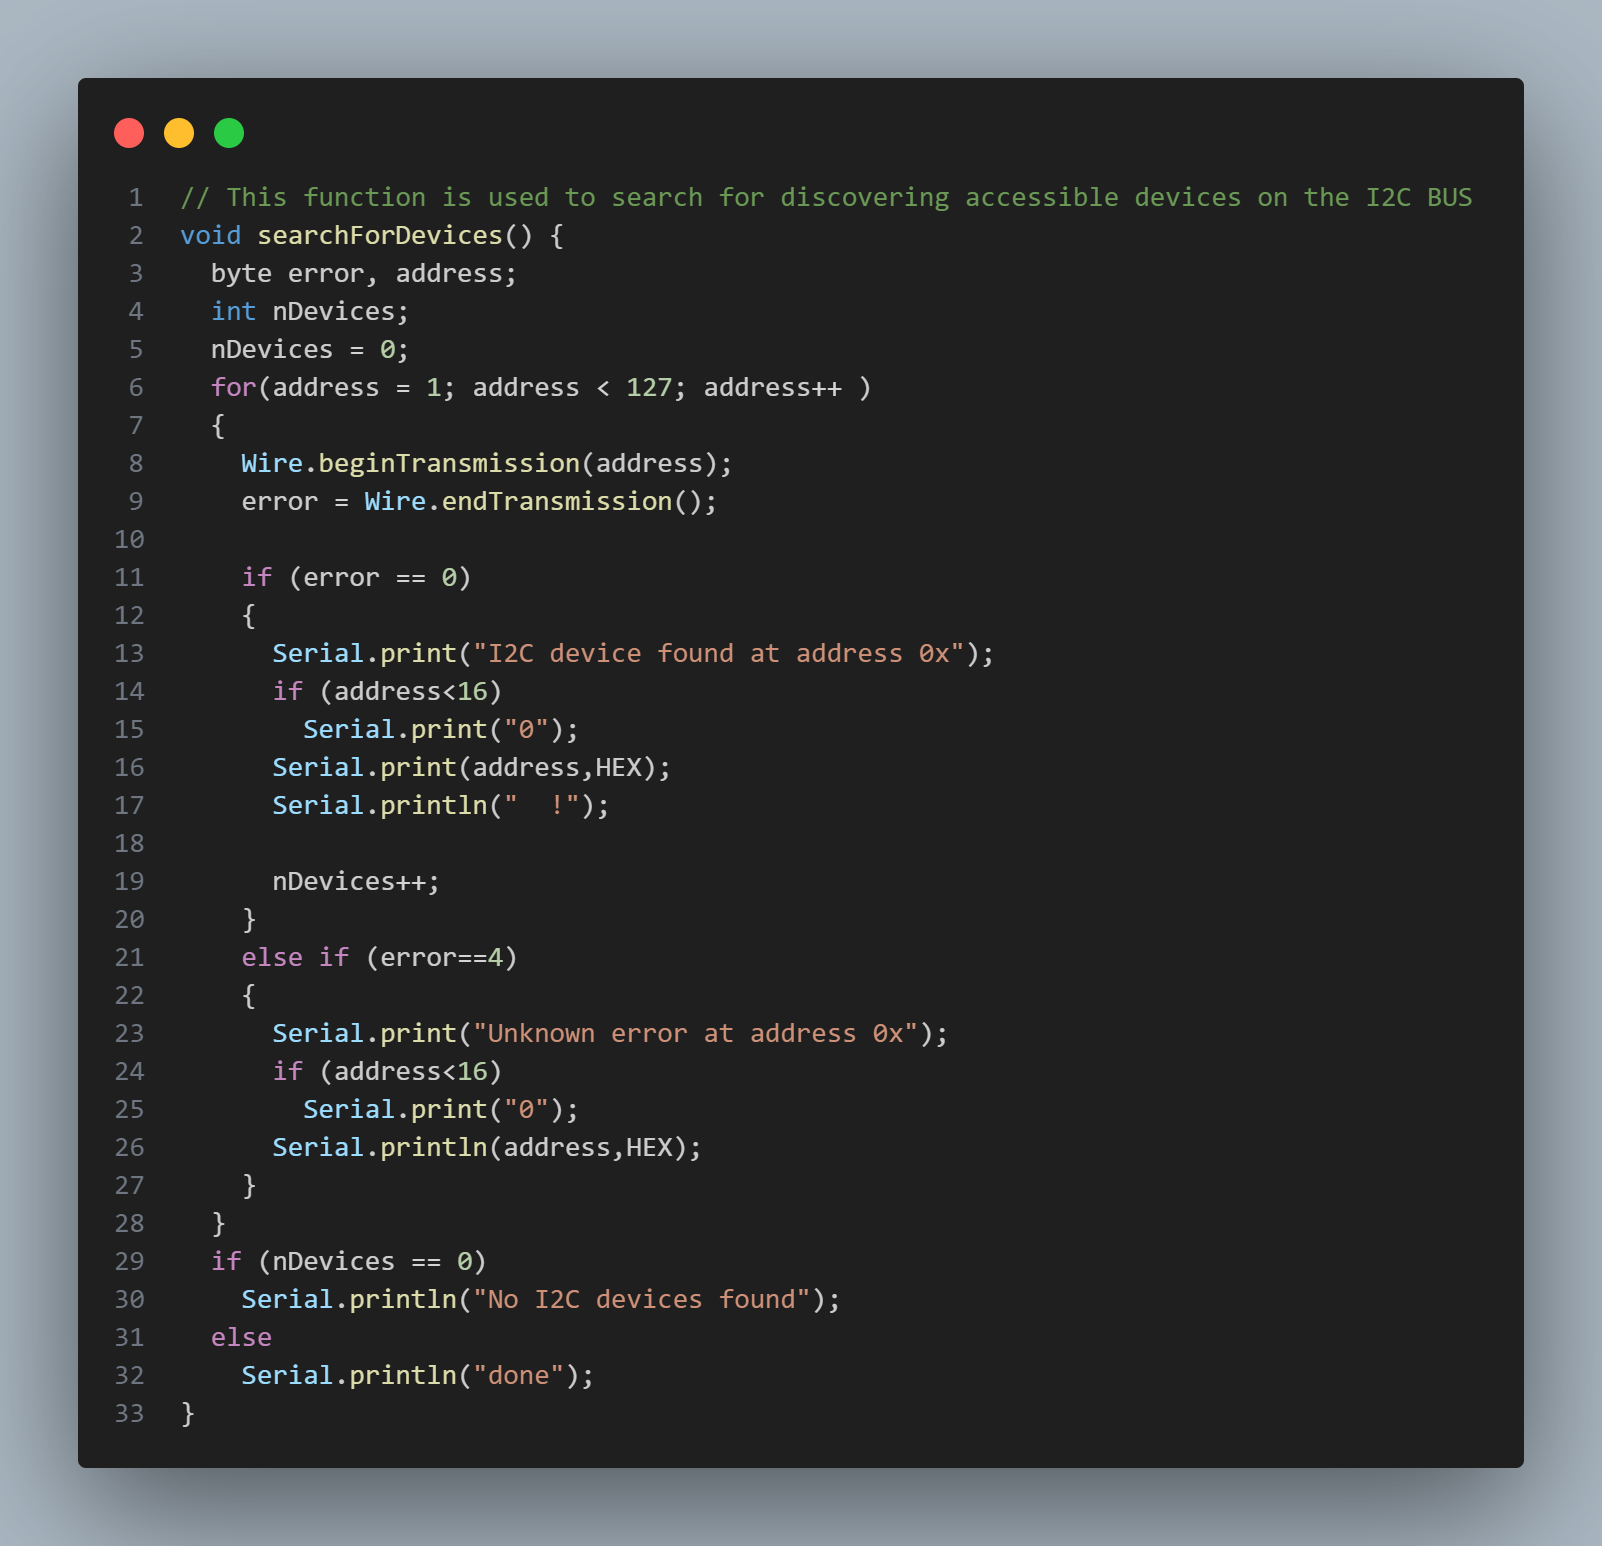
\includegraphics[width=1.0\textwidth]{src/code_snaps/searchDevices.png}
    \caption{Kod źródłowy realizujący wyszukiwanie urządzeń dostępnych na magistrali I2C}
\end{figure}

\subsubsection*{Funkcja \texttt{readFromSensor()}}

Implementacja funkcji czytania wartości z sensora jest bardzo prosrtolinijna. Za pomocą matody \texttt{readRangeContinuousMillimeters()} wywołanej na odpowiednim obiekcie klasy VL53L0X odczytywana jest wartość odległości wyrażona w milimetrach. Jednocześnie odczytana wartość jest przypisywana do odpowiedniej komórki w tablicy pomiarów. 

We fragmencie kodu źródłowego można zauważyć wykomentowany fragment wyświelający wartość odległości. Został on wykorzystany w celu walidacji danych odczytywanych z czujników.

\begin{figure}[H]
    \centering
    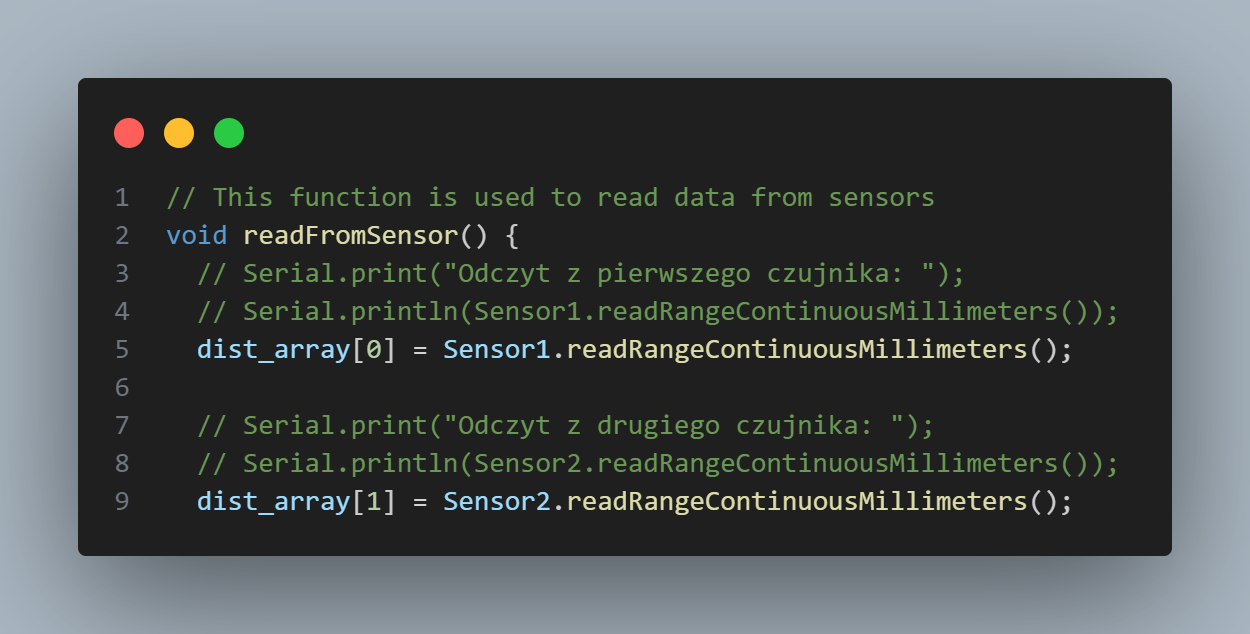
\includegraphics[width=1.0\textwidth]{src/code_snaps/readFromSensor.png}
    \caption{Kod źródłowy realizujący odczytywanie odległości z czujnika}
\end{figure}

\subsubsection*{Funkcja \texttt{processSensorInfo()}}

Powyższa funkcja ma wagę fundamentalną pod kątem poprawności działania robota. Jednocześnie funkcja ta jest najbardziej złożona, przez co zostanie dodany cały kod źródłowy. 

Funkcja rozpoczyna się od inicjalizacji zmiennej \texttt{currentTime()}, jej sens wyjaśni się w miarę zgłębiania logiki wyznacznaia sterowania. 

Pierwsza instrukcja warunkowa sprawdza czy robot znajduje się we wnęce. Stan domyślny jest ustawniony na \texttt{false}. Następnie, zgodnie z dodanymi komentarzami, jeśli przed robotem oraz z prawej strony strony odległość jest większa niż stała \texttt{SAFE\_DIST}, wtedy robot dojedzie do ściany. Funkcja zwraca wartość na podstawie typu wyliczeniowego nadmienionego wcześniej. Dodatkowo w celach pomocniczych wyświetlany jest komunikat o aktualnej trajektorii. 

Następne instrukcje warunkowe realizują sterowanie zgodnie z komentarzami. Warto zwrócić uwagę na instrukcję warunkową rozpoczynającą się w linii 15. Jeśli robot wykryje ścianę przed sobą, robot rozpoczyna ruch w lewo oraz przełącza flagę \texttt{wneka} na wartość \texttt{true}.

Jeśli została wykryta wnęka wykonuje się alternatywna sekwencja instrukcji warunkowych. Jeśli przed robotem ciągle znaduje się przeszkoda, jego ruch pozostaje niezmienny w lewo. W przypadku, gdy czujniki wykryją wolną przestrzeń, włączany jest tryb wyjeżdzania z wnęki. 

Opuszczanie wnęki zostało zrealizowane za pomocą licznika, stąd deklaracja zmiennej \texttt{currentTime} na początku funkcji. W linii nr 55 sprawdzany jest warunek, czy czas przeznaczony na wyjazd z wnęki minął. Jeśli tak, pojazd przełącza się w tryb normalny, jeśli nie, pojazd kontunuuje jazdę prosto. 

Wyjaśnienie wykorzystania takiej struktury zostanie opisane w sekcji 3.3. 

\begin{figure}[H]
    \centering
    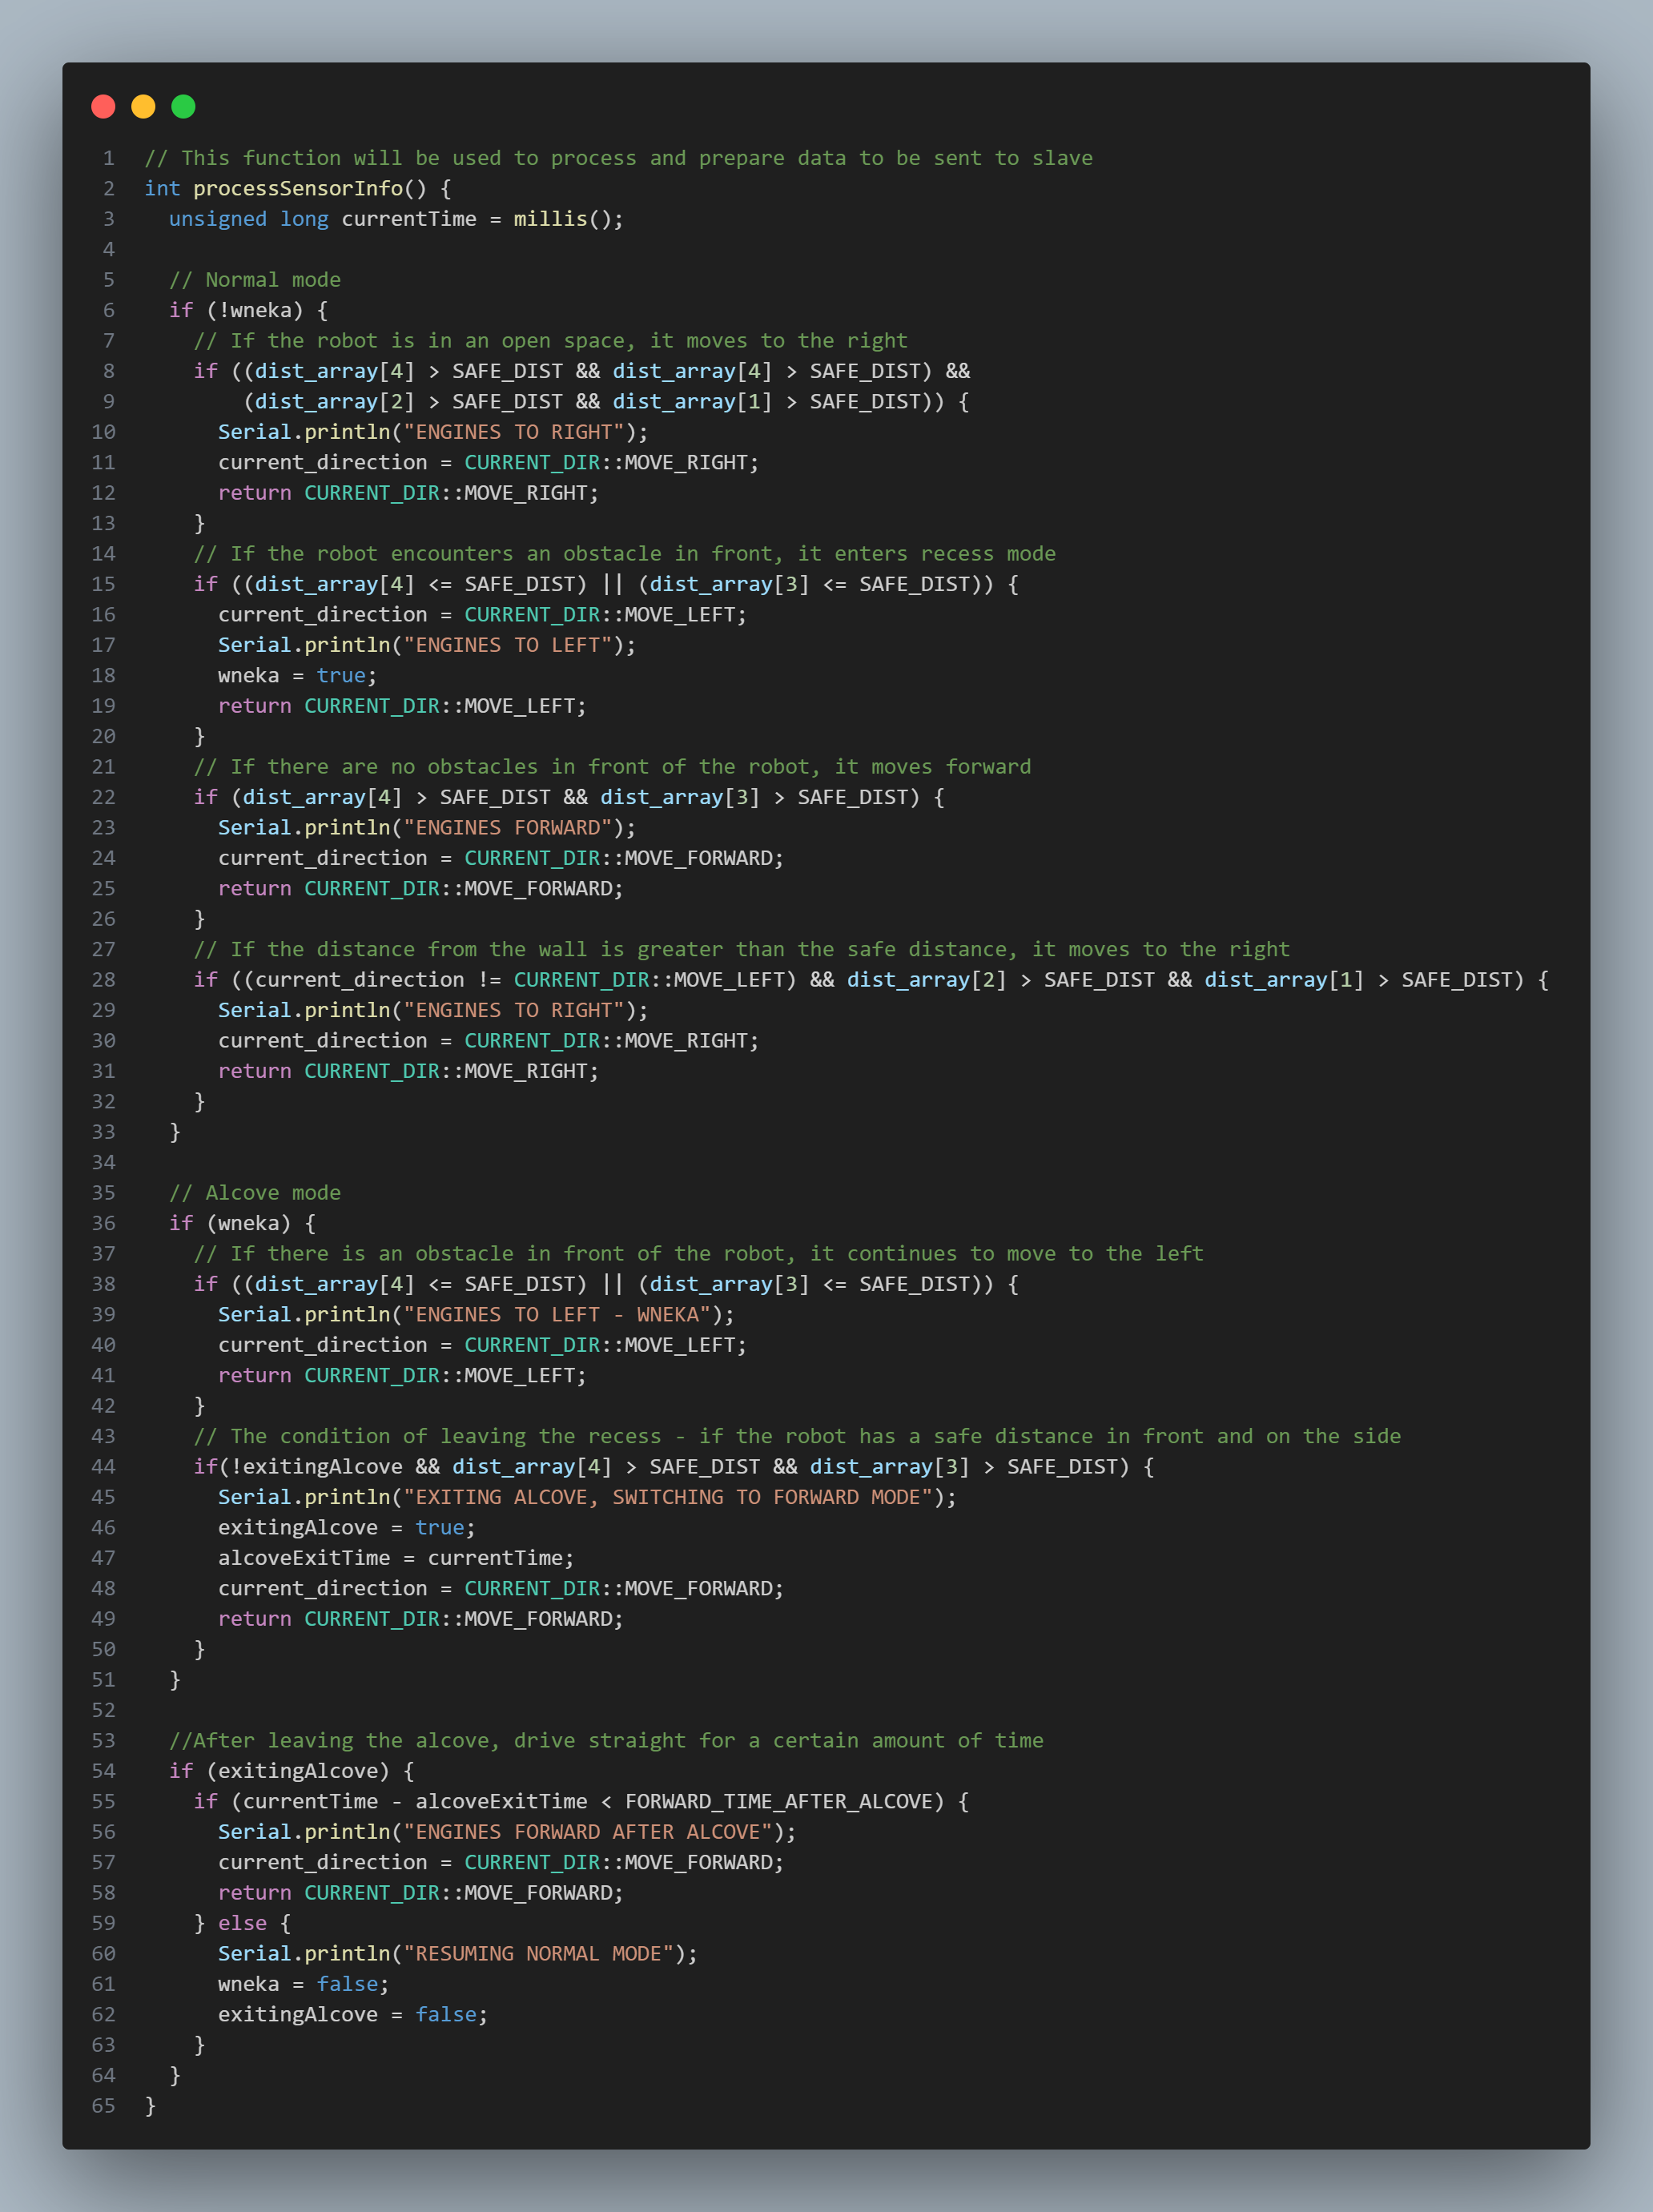
\includegraphics[width=1.0\textwidth]{src/code_snaps/processInfo.png}
    \caption{Kod źródłowy realizujący wyznaczenie odpowiedniego sterowania}
\end{figure}

\newpage

\subsubsection*{Funkcja \texttt{sendSteering()}}

Funkcja ta realizuje wysyłanie wartości odczytanej z funkcji prezetwarzającej dane z sensorów. Pierwszym krokiem jest rozpoczęcie transmisji z urządzeniem o adresie \texttt{0x09} - taki adres jest typowo przydzielany dla drugiego mikrokontrolera Arduino. Następnie za pomocą funkcji \texttt{Wire.write()} odbywa się włąściwy przesył danych poprzez magistralę I2C.

\begin{figure}[H]
    \centering
    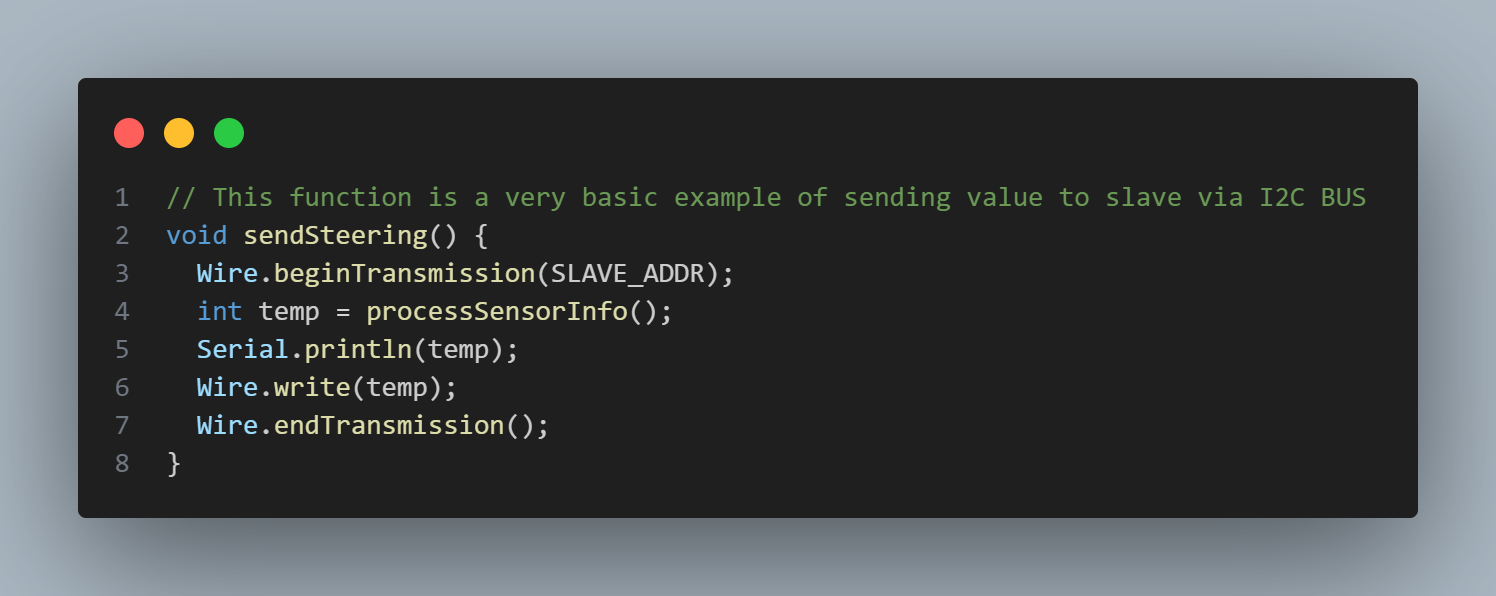
\includegraphics[width=1.0\textwidth]{src/code_snaps/sendSteer.png}
    \caption{Kod źródłowy realizujący wysłanie instrukcji sterowania}
\end{figure}

\subsubsection{\Large Slave}

Mikrokontroler Arduino UNO R3 skonfigurowany do pracy typu Slave odbiera paczkę danych przez zmienną "rd" wysyłane przez Master.

\begin{figure}[H]
    \centering
    \includegraphics*[width=0.4\textwidth]{"src/code_snaps/Comunication_slave.png"}
    \caption{Fragment kodu źródłowego przedstawiający odbiór komunikatów przesyłanych przez mikrokontroler Master.}
    \label{fig:sensor_init}
\end{figure}

Zgodnie z odbieranym komunikatami o zmianie kierunku indeksowanymi od 0 do 3, program wywołuje odpowiednie funkcje. 

\begin{figure}[H]
    \centering
    \includegraphics*[width=0.4\textwidth]{"src/code_snaps/movement_implementation.png"}
    \caption{Fragment kodu źródłowego przedstawiający implementację ruchu pojazdu w odpowiednich kierunkach.}
    \label{fig:sensor_init}
\end{figure}

Funkcje określające kierunek jazdy zostały skonstruowane wedle logiki i geometrii działania kół szwedzkich.

\begin{figure}[H]
    \centering
    \includegraphics*[width=0.7\textwidth]{"src/Robot_pics/Movement.png"}
    \caption{Wizualizacja zależności kierunku jazdy od obrotu kół szwedzkich.}
    \label{fig:sensor_init}
\end{figure}

\subsection{\Large Testy poprawności działania algorytmu sterującego}

% --------------------------------------------------------
% Autor: Wszyscy
%
% TODO: Opisać proces testowania oraz rezultaty algorytmu testującego
%
% Status: 
% --------------------------------------------------------

\section{\LARGE Napotkane problemy}
\subsection{\Large Podłączenie laserowych czujników odległości}
% --------------------------------------------------------
% Autor: Jakub Pająk
%
% TODO: Opisać problemy podczas podłączenia czujników laserowych
%
% Status: 100%
% --------------------------------------------------------

Problematyczne okazało się użytkowanie więcej niż jednego czujnika laserowego przy wykorzystaniu magistrali I2C. Było to spowodowane domyślnytm adresem, który był taki sam dla wszystkich czujników. 

Naturalnym krokiem jest wykorzystanie funkcji \texttt{setAddress()}, ustawiającej inny niż domyślny adres dla czujnika. Niestety wykorzystanie tylko tej funkcji nie przyniosło oczekiwanych rezultatów, w wyniku czego należało szukać rozwiązania dalej. 

Na podstawie dokumentacji oraz informacji znalezionych na forach internetowych, okazało się, że aby z sukcesem zmienić adres czujnika należy wykorzystać dodatkowy pin o nazwie XSHUT. Dzięki niemu czujnik zapamiętywał zmianę adresu i możliwe było wykorzystanie zamierzonej liczby sensorów. 

Dokładny sposób podłączenia czujników oraz wykorzystania pinu XSHUT został opisany w sekcji nr 2.8.

\subsection{\Large Montaż silników oraz kół}
% --------------------------------------------------------
% Autor: Wszyscy
%
% TODO: Opisać problemy podczas montażu
%
% Status: 80%
% --------------------------------------------------------
Pierwszym problemem było zamontowanie samych silników. Okazało się, że dziury na mocowanie silników znajdowały się w innych miejscach niż było to potrzebne. W związku z tym, konieczne było wprowadzenie listwy aluminiowej, która pozwoliła na odpowiednie przymocowanie silników do dolnej części pojazdu.

Kolejnym wyzwaniem było mocowanie kół do silników. Początkowo używaliśmy długich śrub do przymocowania kół, jednak okazało się, że koła były bardzo niestabilnie zamocowane i miały spore luzy. Aby wyeliminować te luzy, wprowadziliśmy boczne listwy aluminiowe, przez które przechodzą długie gwintowane szprychy. To rozwiązanie znacznie poprawiło stabilność kół i zminimalizowało luzy, zapewniając lepsze działanie całego układu.

Dzięki tym działaniom udało się rozwiązać napotkane problemy i zakończyć montaż kół i silników w sposób zapewniający solidność i niezawodność konstrukcji.

\subsection{\Large Implementacja logiki sterowania}
Realizacja logiki realizującej śledzenie ściany bez elementu opuszczania wnęki była realtywnie prosta. Jednak dodanie sekwencji wyjeżdżania z wnęki okazało się wyzwaniem.

Było tak ze względu na kolejność instrukcji warunkowych. Pierwotnie jeśli robot dojeżdzał do ściany jednocześnie mając z prawej swojej strony przeszkodę, poprawnie rozpoczynał ruch w lewo. Jednak po otrzymaniu informacji z sensora o pustej przestrzeni przed, robot od razu rozpoczynał ruch w prawo, ze względu na oddalenie się od prawej strony ściany. W wyniku czego pojazd jeździł tam i z powrotem w kółko. 

Rozwiązaniem okazało się zastosowanie dodatkowego warunku sprawdzającego stan flagi \texttt{wneka} oraz wykorzystanie wymuszonego ruchu do przodu - opisany wcześniej licznik. Dzięki wykorzystaniu wymienionych ulepszeń, robot zarejetrowaniu pustej przestrzeni przed sobą, przez określony czas poruszał się przed siebie, w wyniku czego przynajmniej jeden z czujników z jego prawej strony otrzymywał owartość uniemożliwiającą ruch w prawo. 


\section{\LARGE Podsumowanie}
% --------------------------------------------------------
% Autor: Wszyscy
%
% TODO: Napisać zgrabne podsumowanie projektu, czego się nauczyliśmy oraz sensowne wnioski do popełnionych błędów.
%
% Status: 
% --------------------------------------------------------
\end{document}